\documentclass[10pt,a4paper]{article}
\usepackage[utf8]{inputenc}
\usepackage[spanish]{babel}
\usepackage{amsmath}
\usepackage{amsfonts}
\usepackage{amssymb}
\usepackage{graphicx}
\usepackage{float}
\usepackage[left=2cm,right=2cm,top=2cm,bottom=2cm]{geometry}
\usepackage{circuitikz}
\usepackage{tikz}
\usepackage{tikz-timing}
\usetikztiminglibrary[rising arrows]{clockarrows}
\usepackage{pgfplots}
\pgfplotsset{compat=1.15}
\usetikzlibrary{matrix,calc}
\usepackage{listings}
\usepackage{pdfpages}
\usepackage{lscape}
\usepackage{multicol}
\usepackage{wrapfig}



%isolated term
%#1 - Optional. Space between node and grouping line. Default=0
%#2 - node
%#3 - filling color
\newcommand{\implicantsol}[3][0]{
    \draw[rounded corners=3pt, fill=#3, opacity=0.3] ($(#2.north west)+(135:#1)$) rectangle ($(#2.south east)+(-45:#1)$);
    }


%internal group
%#1 - Optional. Space between node and grouping line. Default=0
%#2 - top left node
%#3 - bottom right node
%#4 - filling color
\newcommand{\implicant}[4][0]{
    \draw[rounded corners=3pt, fill=#4, opacity=0.3] ($(#2.north west)+(135:#1)$) rectangle ($(#3.south east)+(-45:#1)$);
    }

%group lateral borders
%#1 - Optional. Space between node and grouping line. Default=0
%#2 - top left node
%#3 - bottom right node
%#4 - filling color
\newcommand{\implicantcostats}[4][0]{
    \draw[rounded corners=3pt, fill=#4, opacity=0.3] ($(rf.east |- #2.north)+(90:#1)$)-| ($(#2.east)+(0:#1)$) |- ($(rf.east |- #3.south)+(-90:#1)$);
    \draw[rounded corners=3pt, fill=#4, opacity=0.3] ($(cf.west |- #2.north)+(90:#1)$) -| ($(#3.west)+(180:#1)$) |- ($(cf.west |- #3.south)+(-90:#1)$);
}

%group top-bottom borders
%#1 - Optional. Space between node and grouping line. Default=0
%#2 - top left node
%#3 - bottom right node
%#4 - filling color
\newcommand{\implicantdaltbaix}[4][0]{
    \draw[rounded corners=3pt, fill=#4, opacity=0.3] ($(cf.south -| #2.west)+(180:#1)$) |- ($(#2.south)+(-90:#1)$) -| ($(cf.south -| #3.east)+(0:#1)$);
    \draw[rounded corners=3pt, fill=#4, opacity=0.3] ($(rf.north -| #2.west)+(180:#1)$) |- ($(#3.north)+(90:#1)$) -| ($(rf.north -| #3.east)+(0:#1)$);
}

%group corners
%#1 - Optional. Space between node and grouping line. Default=0
%#2 - filling color
\newcommand{\implicantcantons}[2][0]{
    \draw[rounded corners=3pt, opacity=.3] ($(rf.east |- 0.south)+(-90:#1)$) -| ($(0.east |- cf.south)+(0:#1)$);
    \draw[rounded corners=3pt, opacity=.3] ($(rf.east |- 8.north)+(90:#1)$) -| ($(8.east |- rf.north)+(0:#1)$);
    \draw[rounded corners=3pt, opacity=.3] ($(cf.west |- 2.south)+(-90:#1)$) -| ($(2.west |- cf.south)+(180:#1)$);
    \draw[rounded corners=3pt, opacity=.3] ($(cf.west |- 10.north)+(90:#1)$) -| ($(10.west |- rf.north)+(180:#1)$);
    \fill[rounded corners=3pt, fill=#2, opacity=.3] ($(rf.east |- 0.south)+(-90:#1)$) -|  ($(0.east |- cf.south)+(0:#1)$) [sharp corners] ($(rf.east |- 0.south)+(-90:#1)$) |-  ($(0.east |- cf.south)+(0:#1)$) ;
    \fill[rounded corners=3pt, fill=#2, opacity=.3] ($(rf.east |- 8.north)+(90:#1)$) -| ($(8.east |- rf.north)+(0:#1)$) [sharp corners] ($(rf.east |- 8.north)+(90:#1)$) |- ($(8.east |- rf.north)+(0:#1)$) ;
    \fill[rounded corners=3pt, fill=#2, opacity=.3] ($(cf.west |- 2.south)+(-90:#1)$) -| ($(2.west |- cf.south)+(180:#1)$) [sharp corners]($(cf.west |- 2.south)+(-90:#1)$) |- ($(2.west |- cf.south)+(180:#1)$) ;
    \fill[rounded corners=3pt, fill=#2, opacity=.3] ($(cf.west |- 10.north)+(90:#1)$) -| ($(10.west |- rf.north)+(180:#1)$) [sharp corners] ($(cf.west |- 10.north)+(90:#1)$) |- ($(10.west |- rf.north)+(180:#1)$) ;
}

%Empty Karnaugh map 4x4
\newenvironment{Karnaugh}%
{
\begin{tikzpicture}[baseline=(current bounding box.north),scale=0.8]
\draw (0,0) grid (4,4);
\draw (0,4) -- node [pos=0.7,above right,anchor=south west] {cd} node [pos=0.7,below left,anchor=north east] {ab} ++(135:1);
%
\matrix (mapa) [matrix of nodes,
        column sep={0.8cm,between origins},
        row sep={0.8cm,between origins},
        every node/.style={minimum size=0.3mm},
        anchor=8.center,
        ampersand replacement=\&] at (0.5,0.5)
{
                       \& |(c00)| 00         \& |(c01)| 01         \& |(c11)| 11         \& |(c10)| 10         \& |(cf)| \phantom{00} \\
|(r00)| 00             \& |(0)|  \phantom{0} \& |(1)|  \phantom{0} \& |(3)|  \phantom{0} \& |(2)|  \phantom{0} \&                     \\
|(r01)| 01             \& |(4)|  \phantom{0} \& |(5)|  \phantom{0} \& |(7)|  \phantom{0} \& |(6)|  \phantom{0} \&                     \\
|(r11)| 11             \& |(12)| \phantom{0} \& |(13)| \phantom{0} \& |(15)| \phantom{0} \& |(14)| \phantom{0} \&                     \\
|(r10)| 10             \& |(8)|  \phantom{0} \& |(9)|  \phantom{0} \& |(11)| \phantom{0} \& |(10)| \phantom{0} \&                     \\
|(rf) | \phantom{00}   \&                    \&                    \&                    \&                    \&                     \\
};
}%
{
\end{tikzpicture}
}

%Empty Karnaugh map 2x4
\newenvironment{Karnaughvuit}%
{
\begin{tikzpicture}[baseline=(current bounding box.north),scale=0.8]
\draw (0,0) grid (4,2);
\draw (0,2) -- node [pos=0.7,above right,anchor=south west] {bc} node [pos=0.7,below left,anchor=north east] {a} ++(135:1);
%
\matrix (mapa) [matrix of nodes,
        column sep={0.8cm,between origins},
        row sep={0.8cm,between origins},
        every node/.style={minimum size=0.3mm},
        anchor=4.center,
        ampersand replacement=\&] at (0.5,0.5)
{
                      \& |(c00)| 00         \& |(c01)| 01         \& |(c11)| 11         \& |(c10)| 10         \& |(cf)| \phantom{00} \\
|(r00)| 0             \& |(0)|  \phantom{0} \& |(1)|  \phantom{0} \& |(3)|  \phantom{0} \& |(2)|  \phantom{0} \&                     \\
|(r01)| 1             \& |(4)|  \phantom{0} \& |(5)|  \phantom{0} \& |(7)|  \phantom{0} \& |(6)|  \phantom{0} \&                     \\
|(rf) | \phantom{00}  \&                    \&                    \&                    \&                    \&                     \\
};
}%
{
\end{tikzpicture}
}

%Empty Karnaugh map 2x2
\newenvironment{Karnaughquatre}%
{
\begin{tikzpicture}[baseline=(current bounding box.north),scale=0.8]
\draw (0,0) grid (2,2);
\draw (0,2) -- node [pos=0.7,above right,anchor=south west] {b} node [pos=0.7,below left,anchor=north east] {a} ++(135:1);
%
\matrix (mapa) [matrix of nodes,
        column sep={0.8cm,between origins},
        row sep={0.8cm,between origins},
        every node/.style={minimum size=0.3mm},
        anchor=2.center,
        ampersand replacement=\&] at (0.5,0.5)
{
          \& |(c00)| 0          \& |(c01)| 1  \\
|(r00)| 0 \& |(0)|  \phantom{0} \& |(1)|  \phantom{0} \\
|(r01)| 1 \& |(2)|  \phantom{0} \& |(3)|  \phantom{0} \\
};
}%
{
\end{tikzpicture}
}

%Defines 8 or 16 values (0,1,X)
\newcommand{\contingut}[1]{%
\foreach \x [count=\xi from 0]  in {#1}
     \path (\xi) node {\x};
}

%Places 1 in listed positions
\newcommand{\minterms}[1]{%
    \foreach \x in {#1}
        \path (\x) node {1};
}

%Places 0 in listed positions
\newcommand{\maxterms}[1]{%
    \foreach \x in {#1}
        \path (\x) node {0};
}

%Places X in listed positions
\newcommand{\indeterminats}[1]{%
    \foreach \x in {#1}
        \path (\x) node {X};
}


\begin{document}
\begin{titlepage}
\newcommand{\HRule}{\rule{\linewidth}{0.5mm}}
\center
\textsc{\LARGE Instituto Tecnológico de Buenos Aires}\\[1.5cm]
\textsc{\Large 22.13 Electronica III}\\[0.5cm]
\textsc{\large Trabajo Práctico 2}\\[0.5cm]

\HRule \\[0.4cm]
{ \huge \bfseries Tecnología de circuitos lógicos\\Multivibradores\\Contadores secuenciales\\Almacenamiento digital}\\[0.4cm] % Title of your document
\HRule \\[1.5cm]

\begin{minipage}{0.4\textwidth}
\begin{flushleft} \large
\emph{Grupo 4:}\\
Lisandro \textsc{Alvarez} 57.771\\
Milton \textsc{Delgado} 56.451\\
Paulo \textsc{Navarro} 57.775\\
Matias \textsc{Fogg} 56.252\\
\end{flushleft}
\end{minipage}
~
\begin{minipage}{0.4\textwidth}
\begin{flushright} \large
\emph{Profesores:} \\
Kevin \textsc{Dewald}\\
Pablo \textsc{Wundes}
\end{flushright}
\end{minipage}\\[4cm]
% If you don't want a supervisor, uncomment the two lines below and remove the section above %\Large \emph{Author:}\\ %John \textsc{Smith}\\[3cm] % Your name

%{\large \today}\\[3cm] % Date, change the \today to a set date if you want to be precise
\begin{minipage}{0.4\textwidth}
\begin{flushleft} \large
Realizado: 10/10/2018\\
Presentado: 17/10/2018\\
Corrección:\\
\end{flushleft}
\end{minipage}
\vfill % Fill the rest of the page with whitespace

\end{titlepage}


%aca va el ejercicio

Se implementaron dos compuertas NOT con tecnolog�a BJT: una variante con un transistor NPN () y otra con un transistor PNP (). Sus dise�os se pueden observar en la siguiente figura.

%insertar referencias a figuras de dise�o
\begin{figure}[H]% este es para caption arriba o abajo
  \centering
    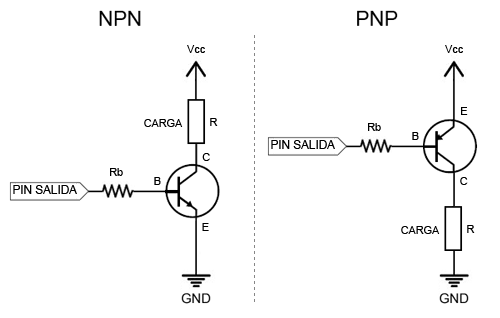
\includegraphics[width=0.5\textwidth]{circuitos}
    \caption{Circuitos inversores para transistores NPN y PNP.} %caption abajo
\end{figure}

Midiendo con un osciloscopio la entrada y la salida del circuito y haciendo uso del modo XY, se obtuvo la curva caracter\'istica de tensi\'on de cada compuerta.

A partir de estas curvas, se obtuvieron los niveles de voltaje de input y output para los niveles altos y bajos de ambas compuertas, as\'i como los m\'argenes de ruido. Estos figuran en la siguiente tabla.
\begin{center}
\begin{table}[H]
\begin{tabular}{|l|l|l|}
\hline
                          & NPN   & PNP    \\
High Level Input Voltage  & 1.18V & 4.28V  \\
Low Level Input Voltage   & 518mV & 3.08V  \\
High Level Output Voltage & 4.88V & 4.53V  \\
Low Level Output Voltage  & 462mV & 12.5mV \\
High Noise Margin         & 3.7V  & 0.25V  \\
Low Noise Margin          & 56mV  & 3.067V
\end{tabular}
\end{table}
\end{center}
Posteriormente, midiendo las curvas de entrada y salida en simult\'aneo, se obtuvieron los tiempos de transici\'on y las demoras de propagaci\'on para ambas compuertas. Luego, se cargaron las compuertas con un capacitor de 10nF, y obteniendo la derivada de la tensi�n de salida, utilizando la ley de Ohm para capacitores pudo determinarse la corriente m\'axima a trav\'es de la compuerta. Estos datos figuran en la siguiente tabla.
\begin{center}
\begin{table}[H]
\begin{tabular}{|l|l|l|}
\hline
                                       & \textbf{NPN} & \textbf{PNP} \\ \hline
\textbf{Propagation Delay High to Low} & 270 ns       & 860 ns       \\ \hline
\textbf{Propagation Delay Low to High} & 3.22 �s      & 101 ns       \\ \hline
\textbf{Transition Time High to Low}   & 230 ns       & 538 ns       \\ \hline
\textbf{Transition Time Low to High}   & 840 ns       & 159 ns       \\ \hline
\textbf{Max Output Current}            & 14.68mA      & 9.25mA       \\ \hline
\end{tabular}
\end{table}
\end{center}

\subsubsection{Mediciones en osciloscopio}
\begin{multicols}{2}
\begin{center}
\begin{figure}[H]% este es para caption arriba o abajo
  \centering
    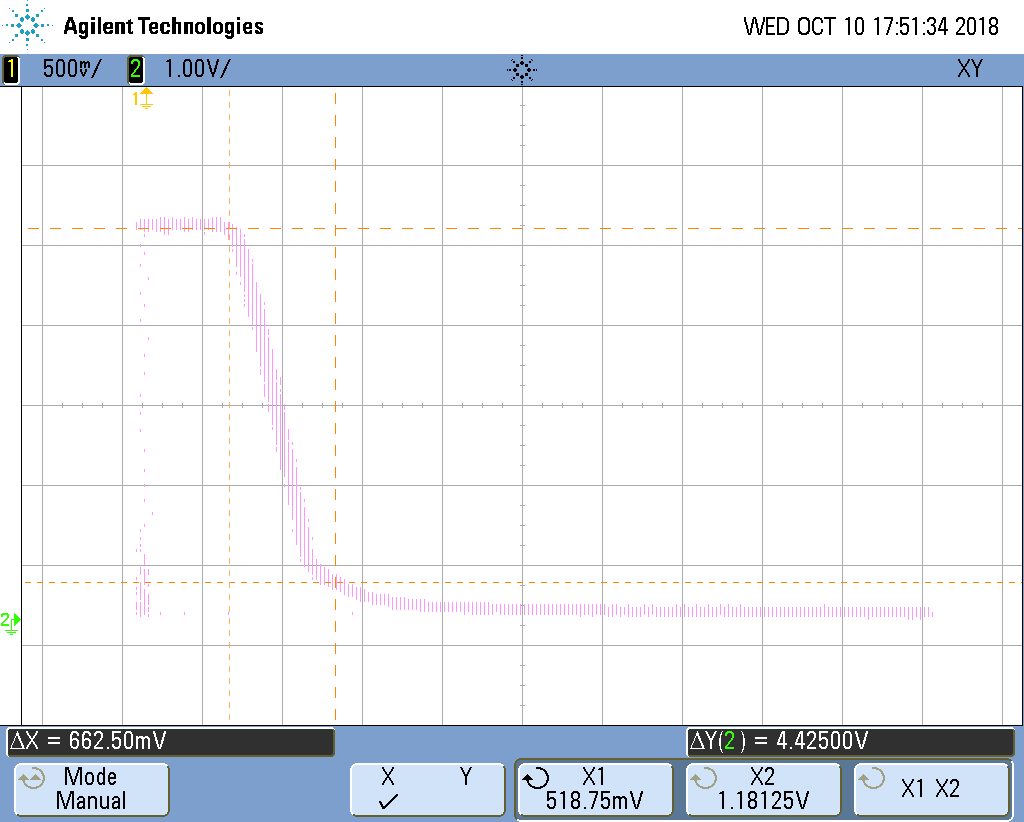
\includegraphics[width=0.4\textwidth]{scope_x_Punto1_NPN}
    \caption{Curva caracter\'istica NPN: datos de input.} %caption abajo
\end{figure}

\begin{figure}[H]% este es para caption arriba o abajo
  \centering
    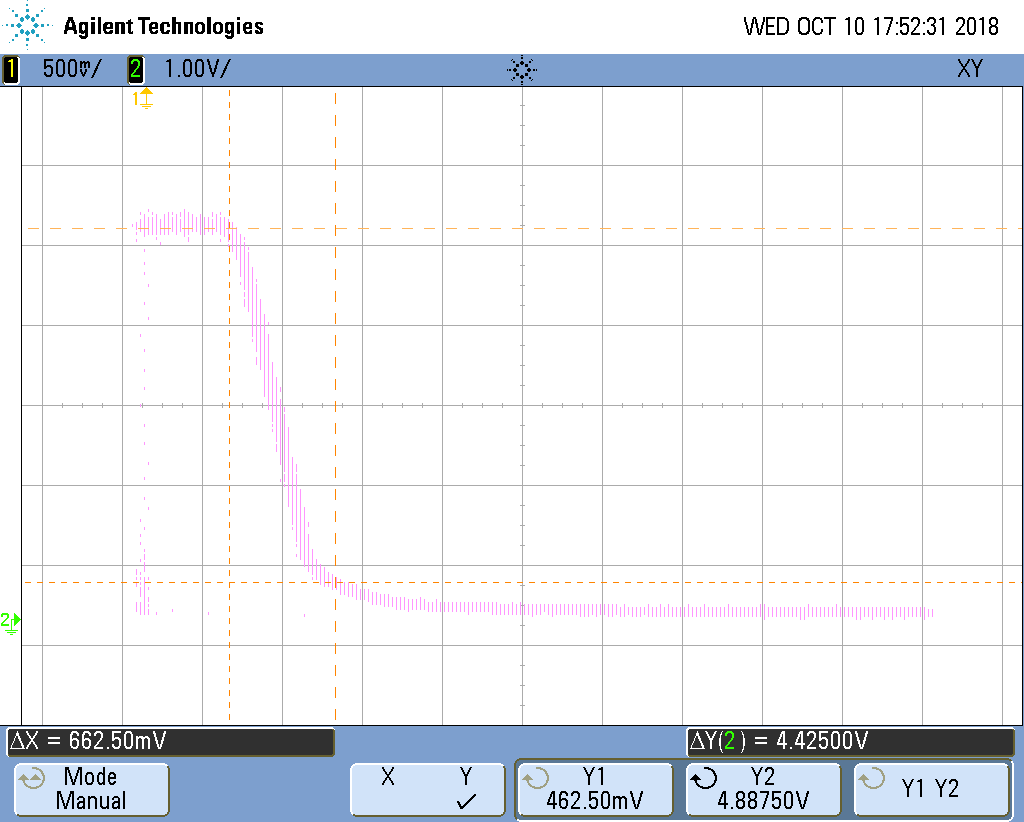
\includegraphics[width=0.4\textwidth]{scope_y_Punto1_NPN}
    \caption{Curva caracter\'istica NPN: datos de output.} %caption abajo
\end{figure}

\begin{figure}[H]% este es para caption arriba o abajo
  \centering
    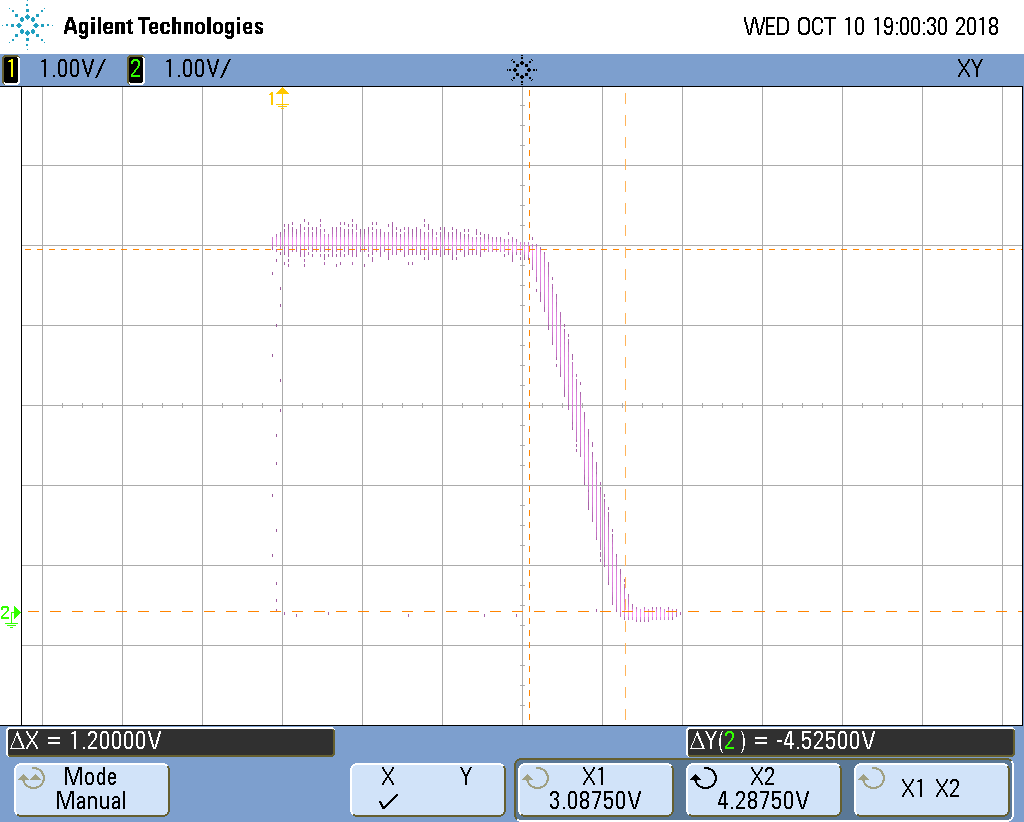
\includegraphics[width=0.4\textwidth]{scope_x_Punto1_PNP}
    \caption{Curva caracter\'istica PNP: datos de input.} %caption abajo
\end{figure}

\begin{figure}[H]% este es para caption arriba o abajo
  \centering
    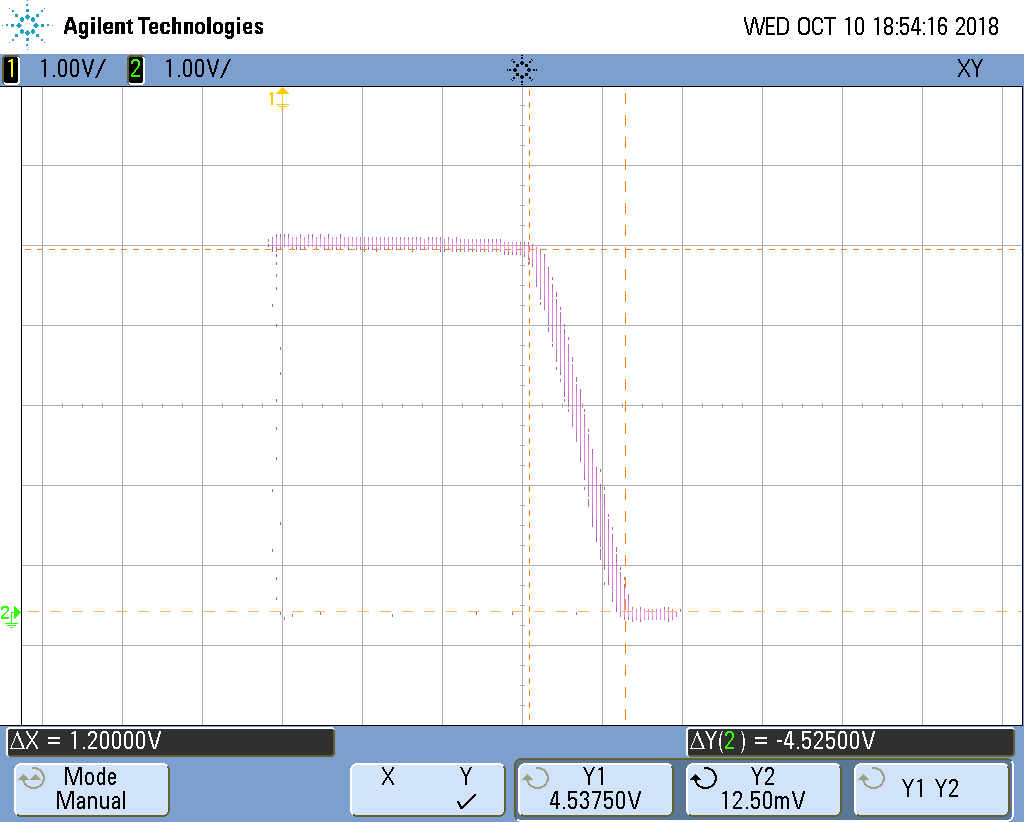
\includegraphics[width=0.4\textwidth]{scope_y_Punto1_PNP}
    \caption{Curva caracter\'istica PNP: datos de output.} %caption abajo
\end{figure}

\begin{figure}[H]% este es para caption arriba o abajo
  \centering
    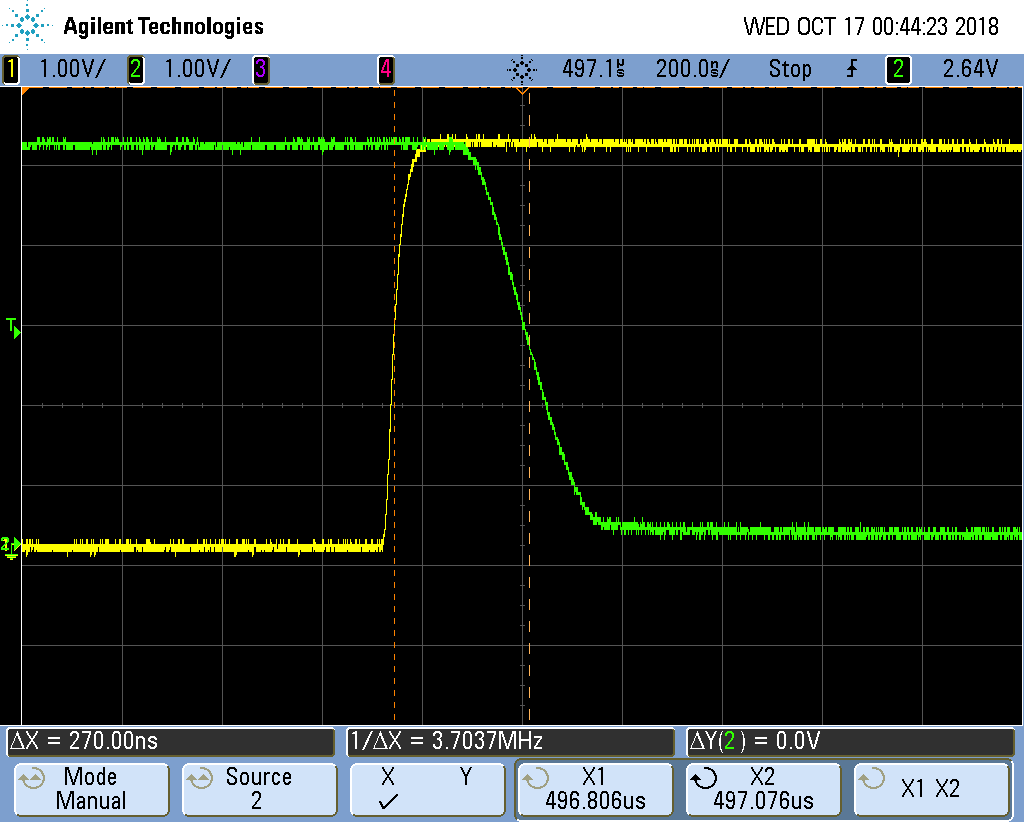
\includegraphics[width=0.4\textwidth]{pHL-NPN}
    \caption{Medici\'on Propagation Delay NPN: High to Low} %caption abajo
\end{figure}

\begin{figure}[H]% este es para caption arriba o abajo
  \centering
    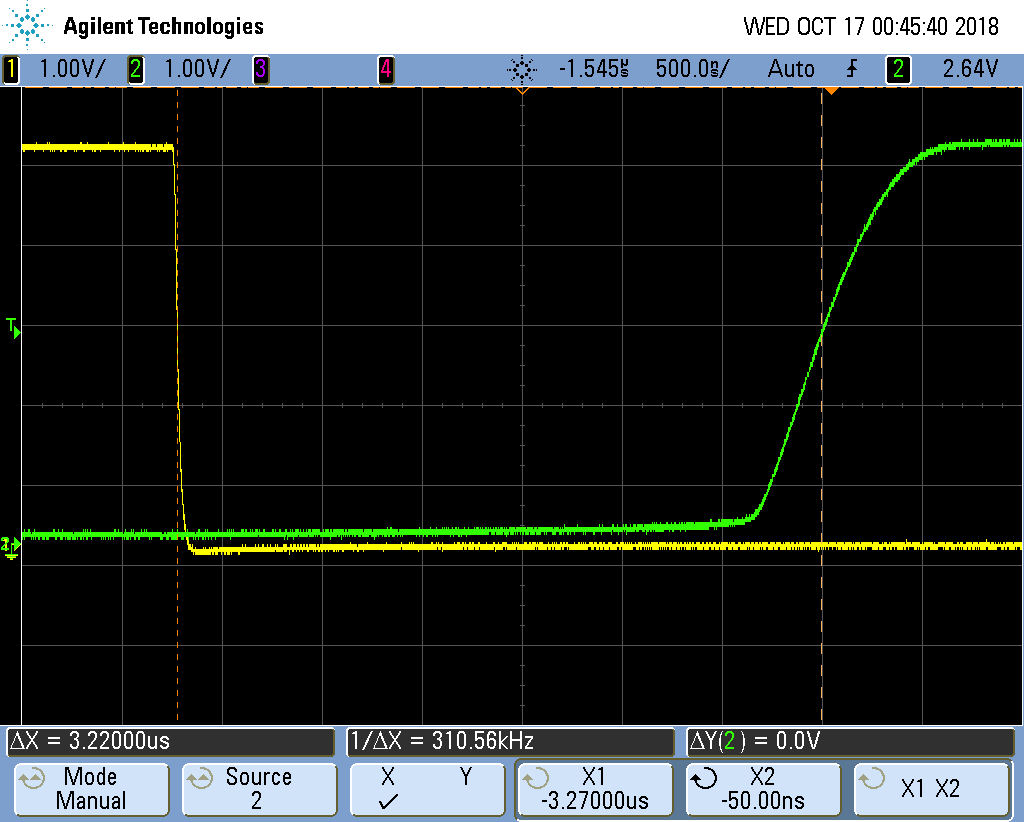
\includegraphics[width=0.4\textwidth]{pLH-NPN}
    \caption{Medici\'on Propagation Delay NPN: Low to High} %caption abajo
\end{figure}

\begin{figure}[H]% este es para caption arriba o abajo
  \centering
    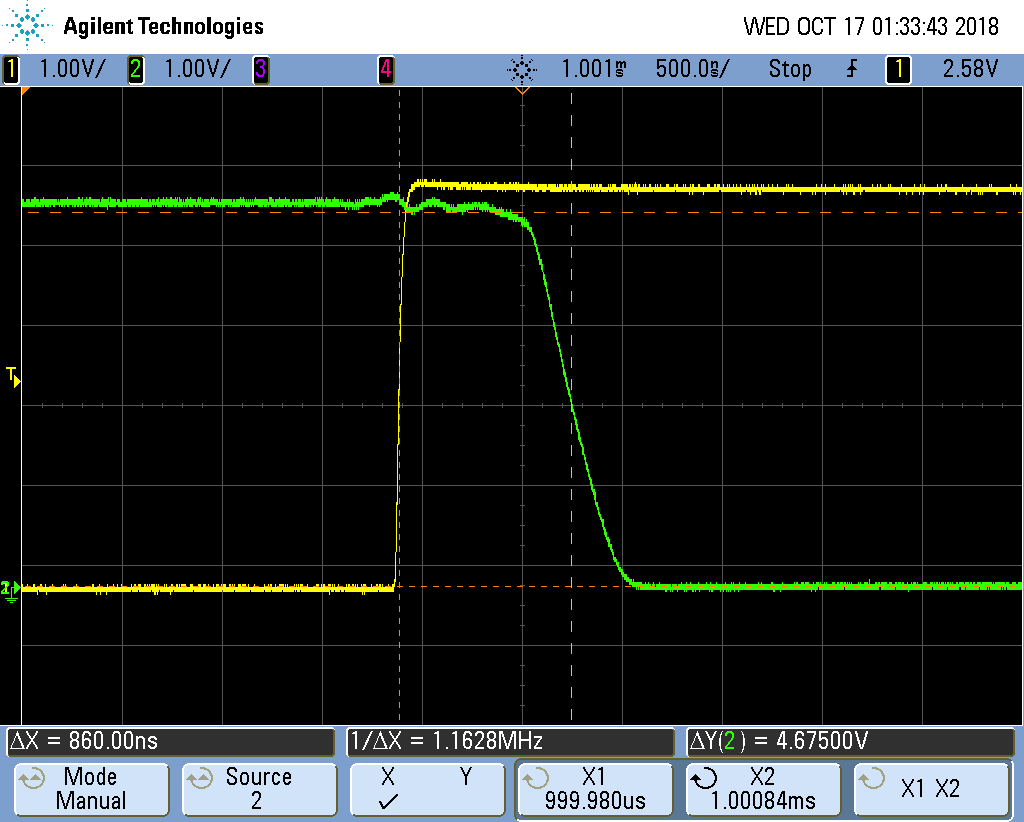
\includegraphics[width=0.4\textwidth]{pHL-PNP}
    \caption{Medici\'on Propagation Delay PNP: High to Low} %caption abajo
\end{figure}

\begin{center}
\begin{figure}[H]% este es para caption arriba o abajo
  \centering
    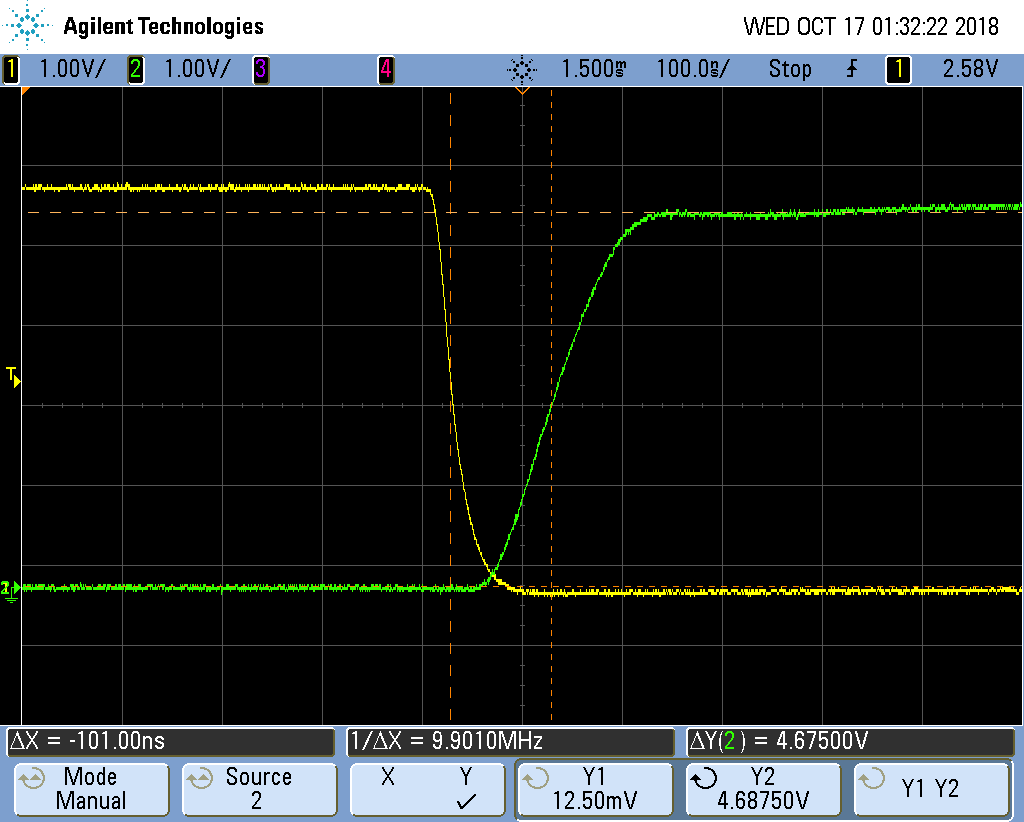
\includegraphics[width=0.4\textwidth]{pLH-PNP}
    \caption{Medici\'on Propagation Delay PNP: Low to High} %caption abajo
\end{figure}

\begin{figure}[H]% este es para caption arriba o abajo
  \centering
    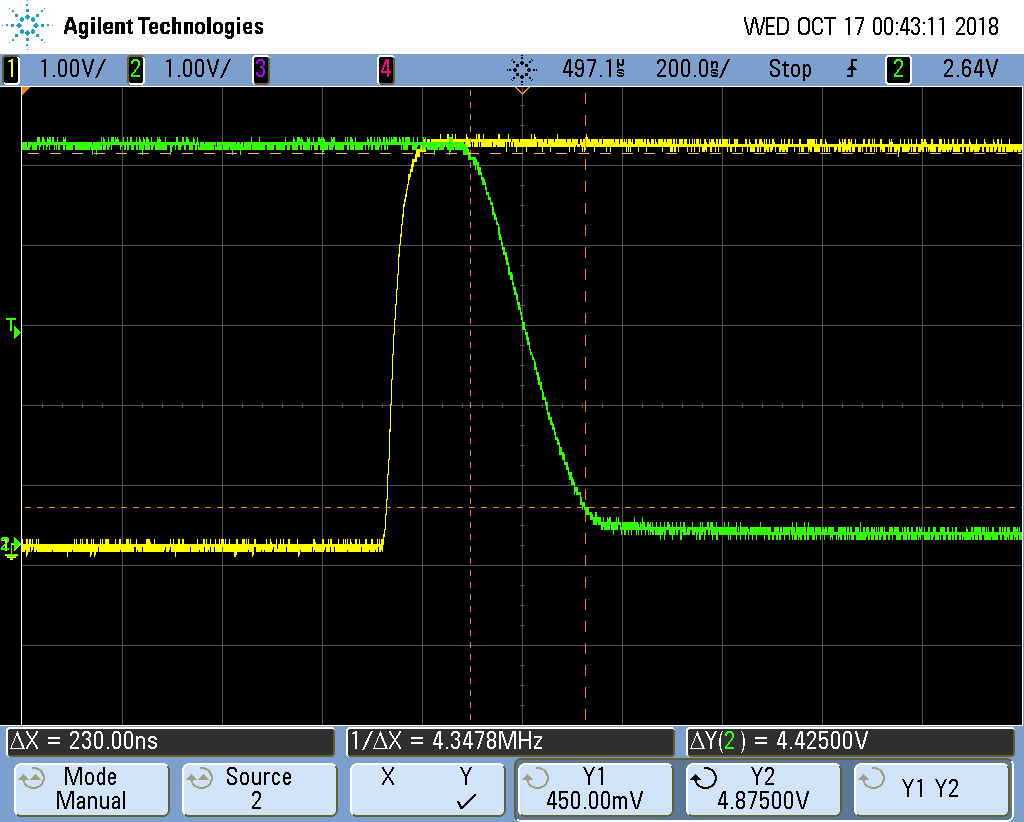
\includegraphics[width=0.4\textwidth]{tHL-NPN}
    \caption{Medici\'on Transition Time NPN: High to Low} %caption abajo
\end{figure}

\begin{figure}[H]% este es para caption arriba o abajo
  \centering
    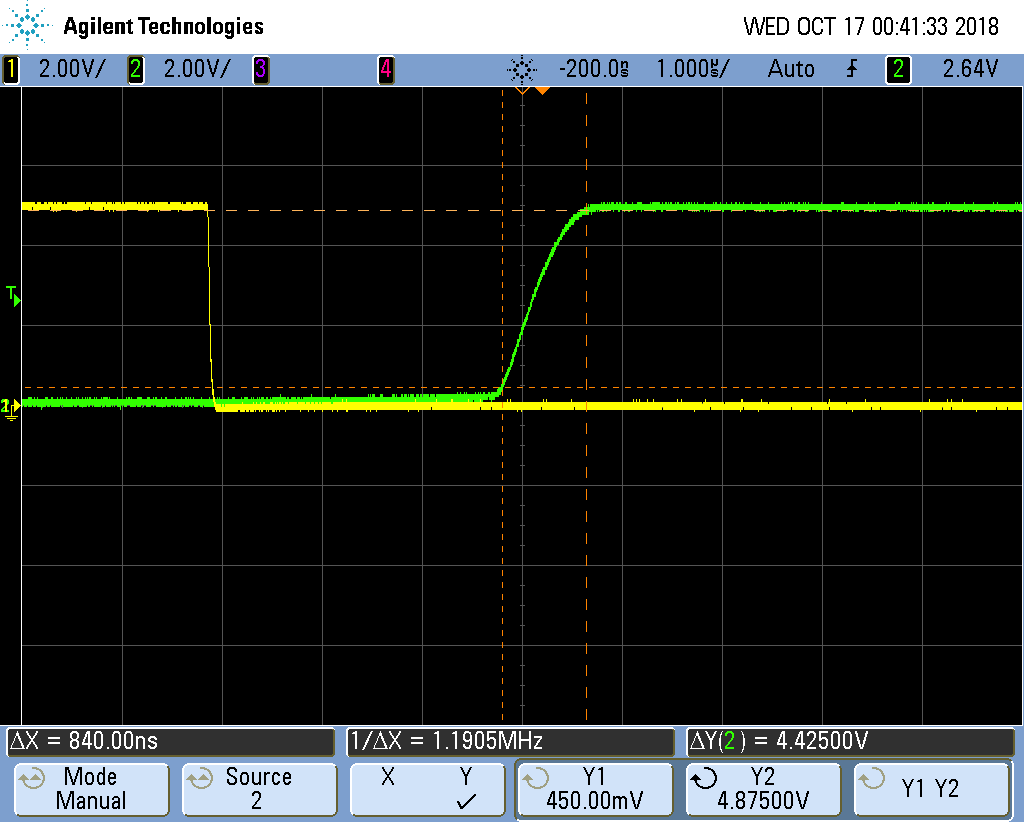
\includegraphics[width=0.4\textwidth]{tLH-NPN}
    \caption{Medici\'on Transition Time NPN: Low to High} %caption abajo
\end{figure}

\begin{figure}[H]% este es para caption arriba o abajo
  \centering
    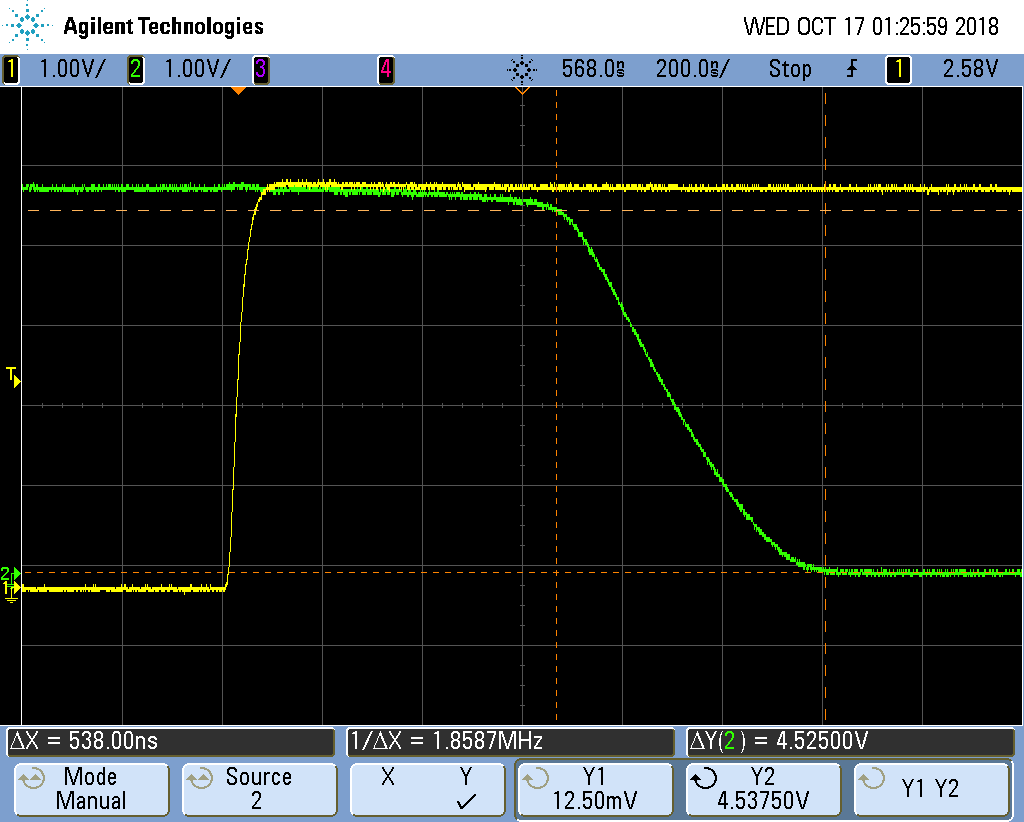
\includegraphics[width=0.4\textwidth]{tHL-PNP}
    \caption{Medici\'on Transition Time PNP: High to Low} %caption abajo
\end{figure}

\begin{figure}[H]% este es para caption arriba o abajo
  \centering
    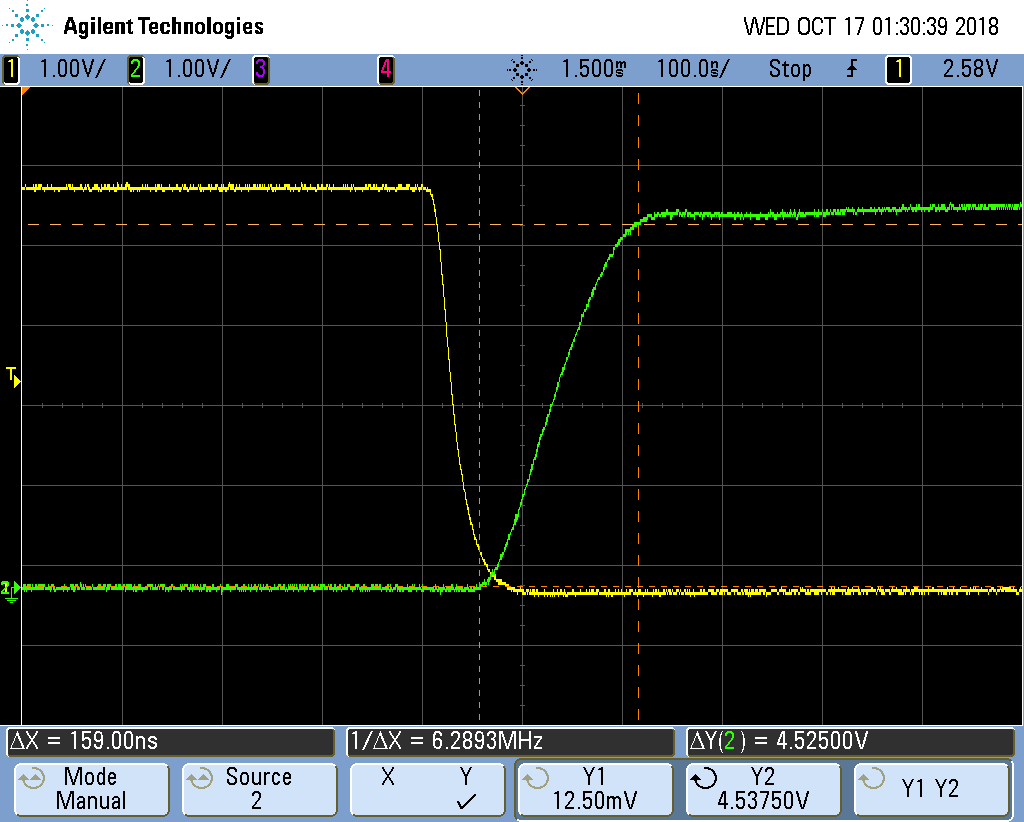
\includegraphics[width=0.4\textwidth]{tLH-PNP}
    \caption{Medici\'on Transition Time PNP: Low to High} %caption abajo
\end{figure}

\begin{figure}[H]% este es para caption arriba o abajo
  \centering
    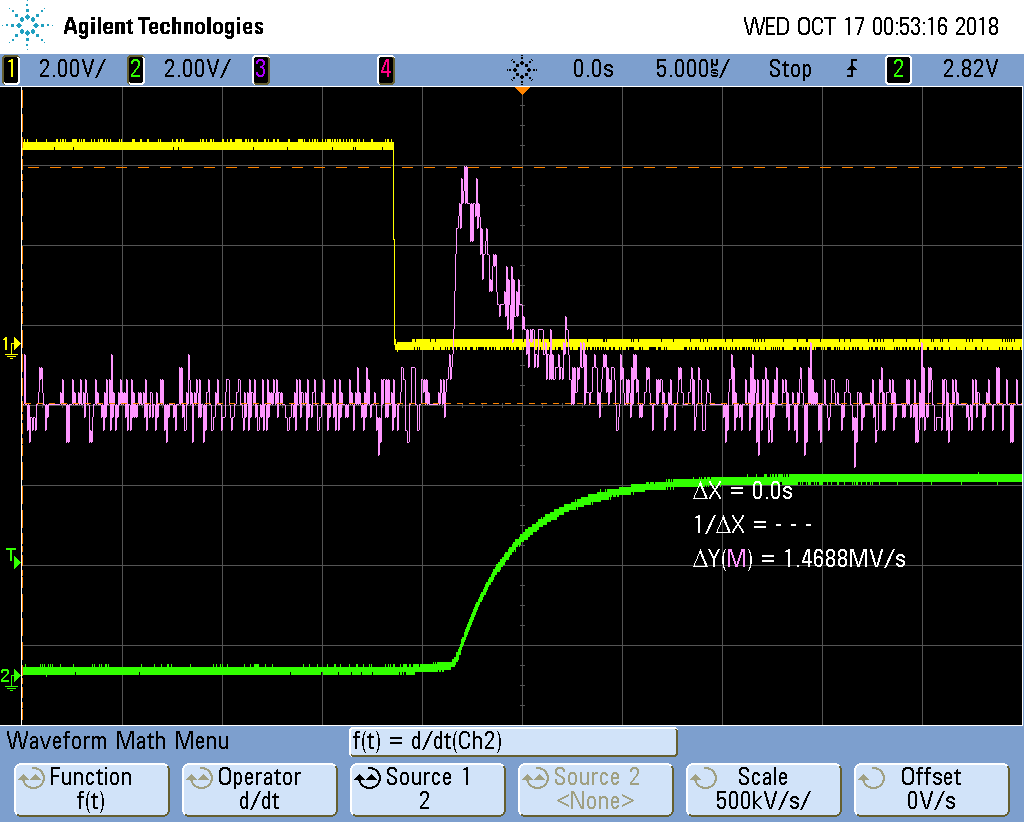
\includegraphics[width=0.4\textwidth]{maxI-NPN}
    \caption{Medici\'on m�xima derivada de tensi�n en la salida NPN} %caption abajo
\end{figure}

\begin{figure}[H]% este es para caption arriba o abajo
  \centering
    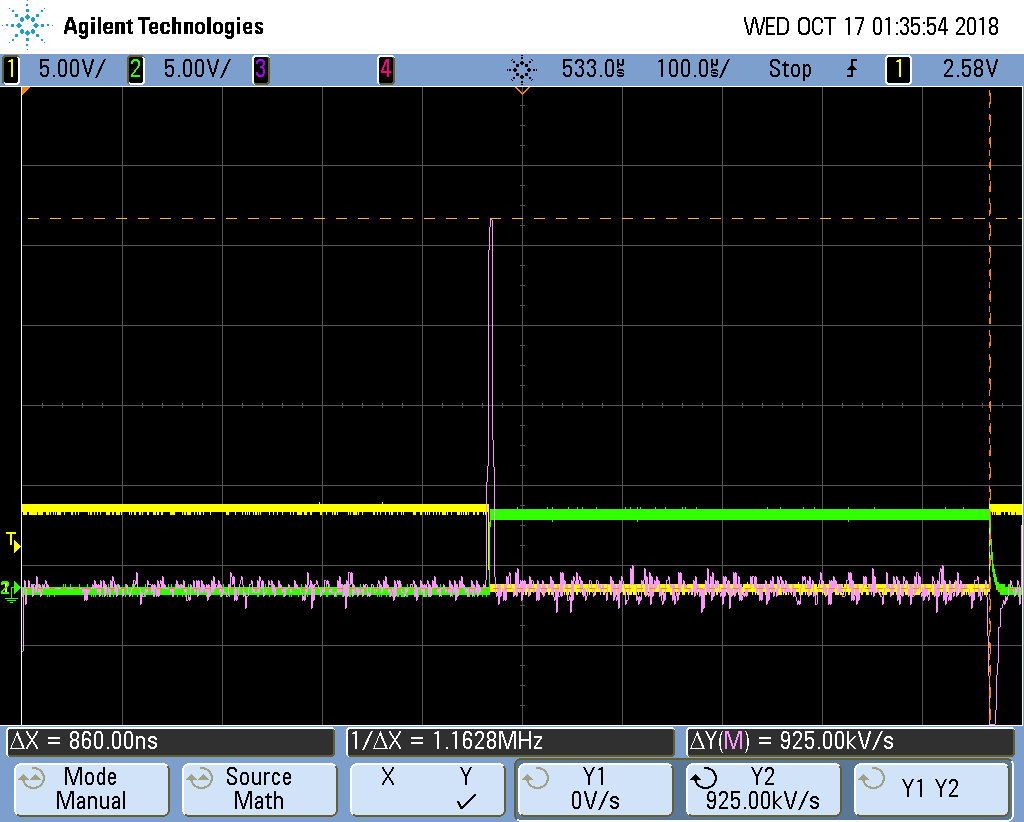
\includegraphics[width=0.4\textwidth]{maxI-PNP}
    \caption{Medici\'on m�xima derivada de tensi�n en la salida PNP} %caption abajo
\end{figure}
\end{center}
\end{multicols}
\iffalse
Seccion de cosas utiles para agregar

texto----------------------------
\textit[texto en negrita]




listas --------------------------------------------------
\begin{list_type}  
\item The first item 
\item The second item 
\item The third etc \ldots 
\end{list_type}

list_type es:
itemize for a bullet list
enumerate for an enumerated list and
description for a descriptive list.

ejemplo listas anidadas-----------------------------------------------

\begin{enumerate}
\item The first item
\begin{enumerate}
\item Nested item 1
\item Nested item 2
\end{enumerate}
\item The second item
\item The third etc \ldots
\end{enumerate}

tildes-------------------------------
babel ya esta incluido, si hay que poner tildes se ponen \acute{i}
ejemplo: l\acute{i}mite

tip: escriban normal y despues hagan replace

subsecciones-------------------------------

si necesitan subsecciones le clavan un buen \subsection*{nombre}

y si estan en piolas y necesitan sub sub secciones le clavan un \subsubsection*{nombre}

quien hubiera dicho

figuras----------------------------------------

\begin{figure}% este es para caption arriba o abajo
  \caption{A picture of a gull.} %caption arriba
  \centering
    \includegraphics[width=0.5\textwidth]{gull}
    \caption{A picture of a gull.} %caption abajo
\end{figure}

\begin{SCfigure} %este es para caption al costado
  \centering
  \caption{ ... caption text ... } 
  \includegraphics[width=0.3\textwidth]%
    {Giraffe_picture}% picture filename
\end{SCfigure}

para hacer que la figure se quede quietecita:

\begin{figure}[letrita_placement]

donde letrita_placement es:
h	Place the float here, i.e., approximately at the same point it occurs in the source text (however, not exactly at the spot)
t	Position at the top of the page.
b	Position at the bottom of the page.
p	Put on a special page for floats only.
!	Override internal parameters LaTeX uses for determining "good" float positions.
H	Places the float at precisely the location in the LaTeX code. Requires the float package,[1] i.e., \usepackage{float}. This is somewhat equivalent to !ht.

\fi
\part*{Ejercicio 2}

Se tomaron los datos de m\'aximos y m\'inimos de las entradas y salidas para los distintos estados de las hojas de datos de los circuitos en cuesti\'on, y se exhiben en el cuadro \ref{tab:datos74}.
\begin{table}[H]
\begin{tabular}{|l|l|l|l|l|l|l|}
\hline
                                                                            & Vcc                                                        & Voltage (25 C)                                              & Vcc         & Voltage (25 C) & Vcc      & Voltage (25 C)   \\ \hline
                                                                      & \multicolumn{2}{l|}{74HC02}                                                                                              & \multicolumn{2}{l|}{74HCT02} & \multicolumn{2}{l|}{74LS02} \\ \hline
\begin{tabular}[c]{@{}l@{}}Minimum HIGH Level\\ Input Voltage\end{tabular}  & \begin{tabular}[c]{@{}l@{}}2.0V\\ 4.5V\\ 6.0V\end{tabular} & \begin{tabular}[c]{@{}l@{}}1.5V\\ 3.15V\\ 4.2V\end{tabular} & 4.5V a 5.5V & 2V             & 4.75V    & 2V               \\ \hline
\begin{tabular}[c]{@{}l@{}}Maximum LOW Level\\ Input Voltage\end{tabular}   & \begin{tabular}[c]{@{}l@{}}2.0V\\ 4.5V\\ 6.0V\end{tabular} & \begin{tabular}[c]{@{}l@{}}0.5V\\ 1.35V\\ 1.8V\end{tabular} & 4.5V a 5.5V & 0.8V           & 4.75V    & 0.8V             \\ \hline
\begin{tabular}[c]{@{}l@{}}Minimum HIGH Level\\ Output Voltage\end{tabular} & \begin{tabular}[c]{@{}l@{}}2.0V\\ 4.5V\\ 6.0V\end{tabular} & \begin{tabular}[c]{@{}l@{}}1.9V\\ 4.4V\\ 5.9V\end{tabular}  & 4.5V a 5.5V & 4.4V           & 4.75V    & 2.7V             \\ \hline
\begin{tabular}[c]{@{}l@{}}Maximum LOW Level\\ Output Voltage\end{tabular}  & \begin{tabular}[c]{@{}l@{}}2.0V\\ 4.5V\\ 6.0V\end{tabular} & \begin{tabular}[c]{@{}l@{}}0.1V\\ 0.1V\\ 0.1V\end{tabular}  & 4.5V a 5.5V & 0.1V           & 4.75V    & 0.5V             \\ \hline
\end{tabular}
\caption{Tabla de informaci\'on obtenida de las hojas de datos}
\label{tab:datos74}
\end{table}

Como se ilustra en las figuras para los cuatro casos planteados, s\'olo habr\'ia problemas si se intenta conectar un transistor HC a la salida de un LS: la salida alta del LS puede caer en la regi\'on indeterminada de la entrada del HC, y sin que falle ning\'un componente fallar\'ia el circuito.

En todos los dem\'as casos se genera un margen de error para las entradas de los transistores.

\begin{figure}[H]
\begin{center}
  \begin{minipage}[b]{0.4\textwidth}
  	\begin{center}
  		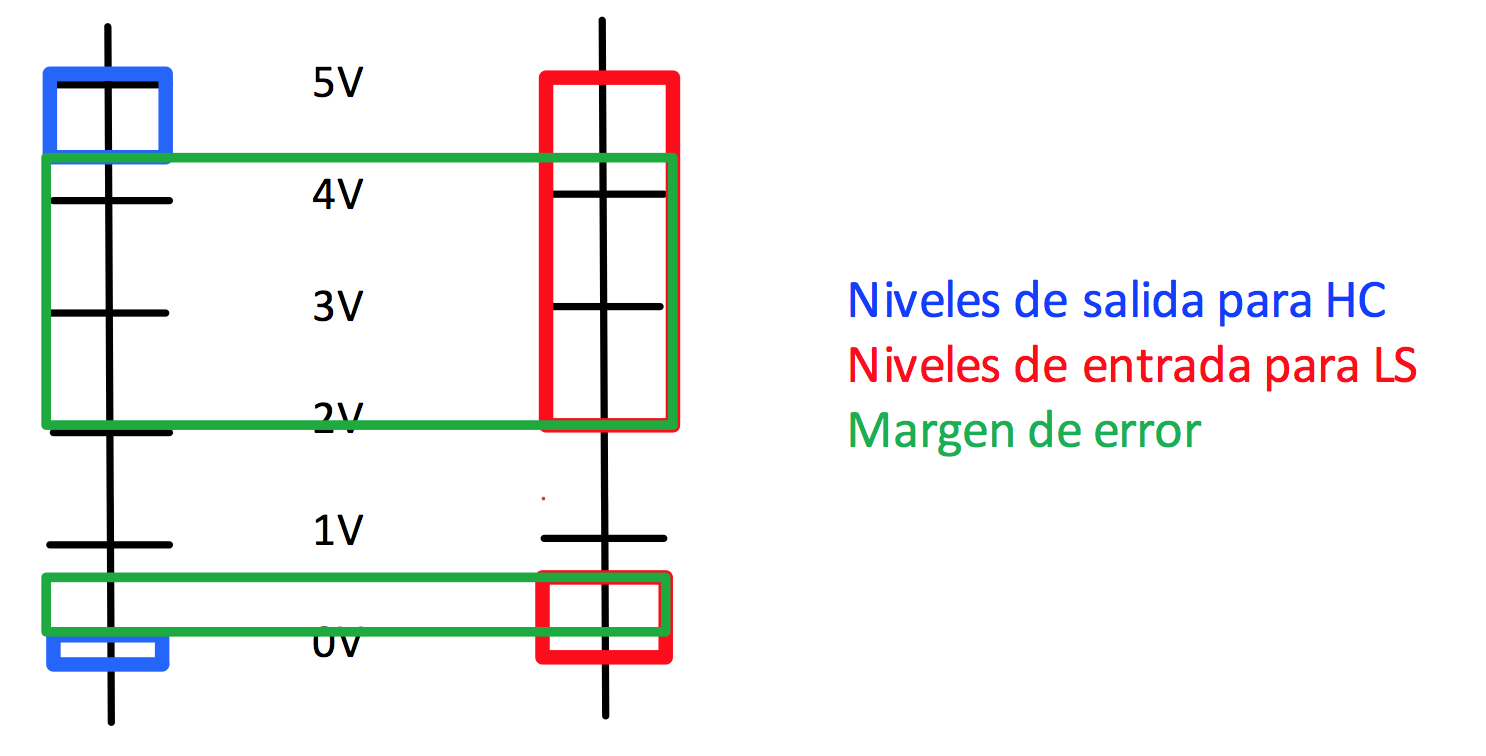
\includegraphics[width=6cm]{ejercicio2/HC-LS}
    \caption{Niveles de tensi\'on para caso HC alimenta a LS.} %caption abajo
  	\end{center}
  \caption{Circuito utilizado}
  \label{7_fig1}
  \end{minipage}
  \begin{minipage}[b]{0.4\textwidth}
    \begin{center}
  		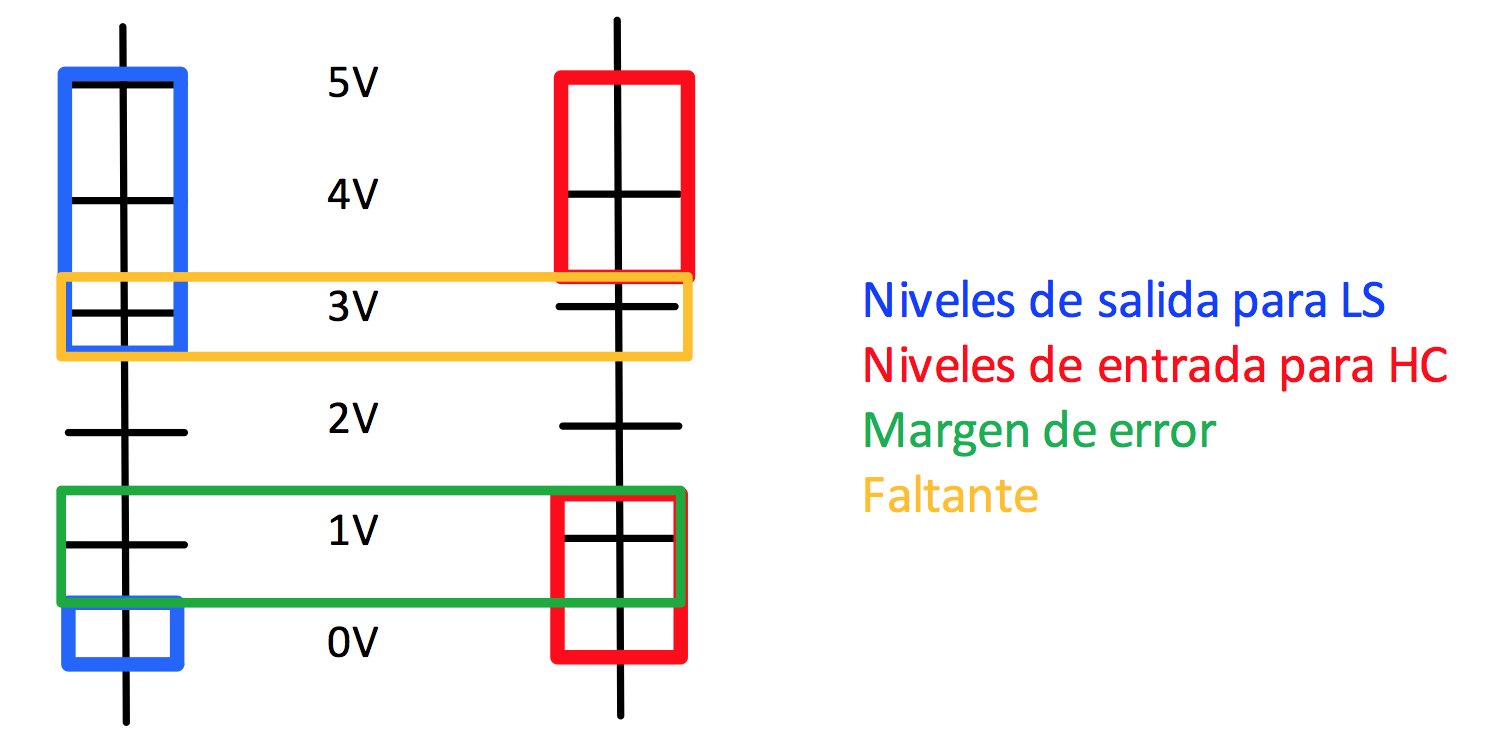
\includegraphics[width=6cm]{ejercicio2/LS-HC}
    \caption{Niveles de tensi\'on para caso LS alimenta a HC.} %caption abajo
	\end{center}
  \caption{Implementaci\'on con 74HC112}
  \label{7_fig2}
 \end{minipage}
\end{center}
\end{figure}


\begin{figure}[H]
\begin{center}
  \begin{minipage}[b]{0.4\textwidth}
  	\begin{center}
  		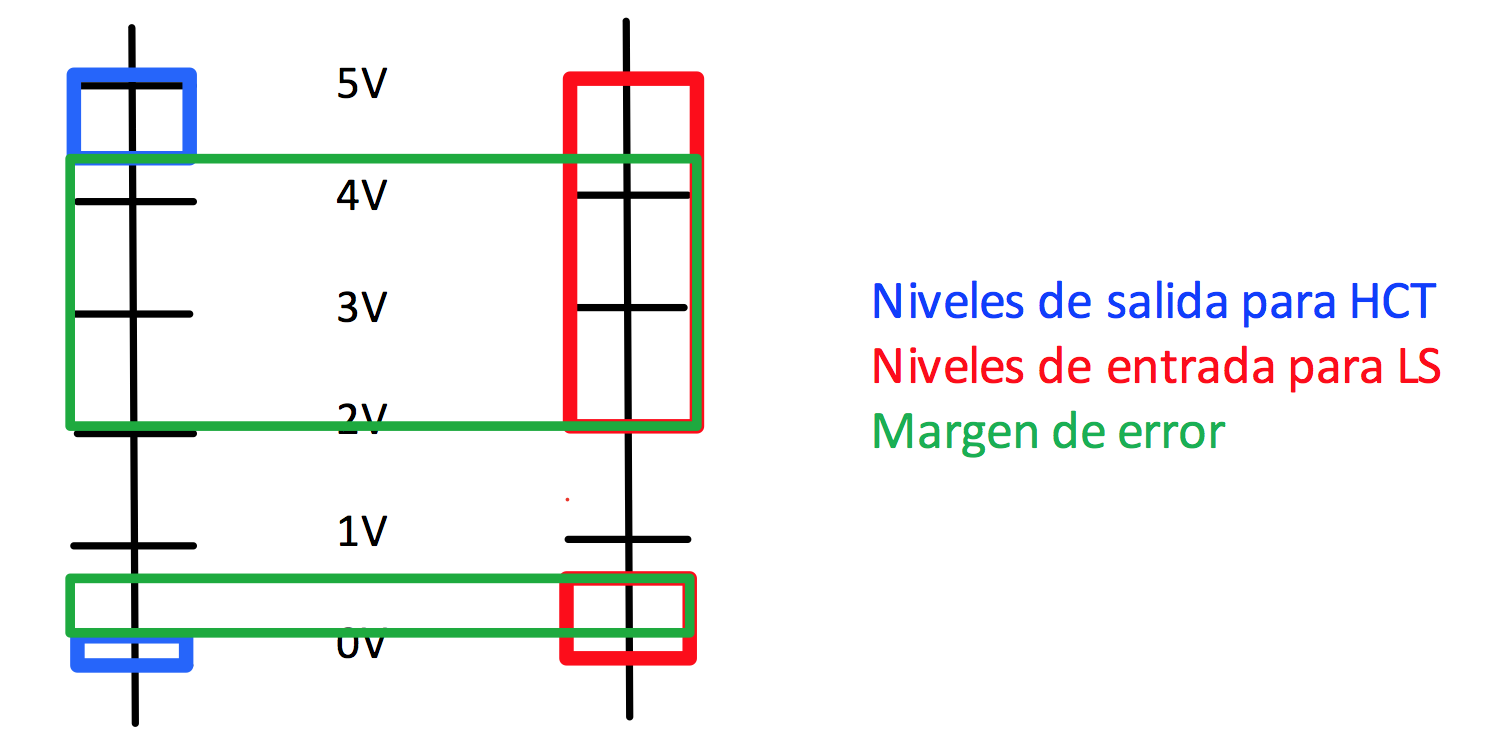
\includegraphics[width=6cm]{ejercicio2/HCT-LS}
    \caption{Niveles de tensi\'on para caso HCT alimenta a LS.} %caption abajo
  	\end{center}
  \caption{Circuito utilizado}
  \label{7_fig1}
  \end{minipage}
  \begin{minipage}[b]{0.4\textwidth}
    \begin{center}
  		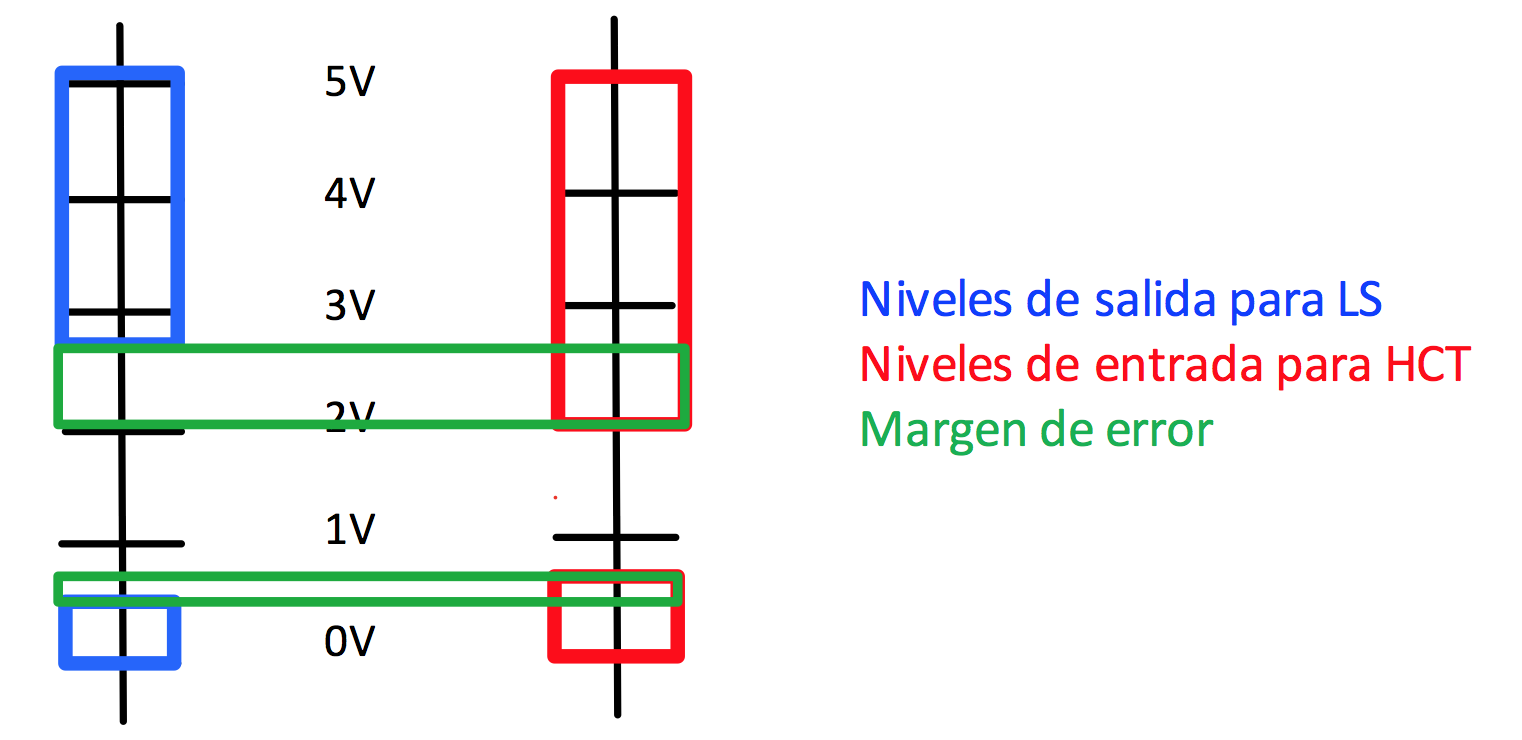
\includegraphics[width=6cm]{ejercicio2/LS-HCT}
    \caption{Niveles de tensi\'on para caso LS alimenta a HCT.} %caption abajo
	\end{center}
  \caption{Implementaci\'on con 74HC112}
  \label{7_fig2}
 \end{minipage}
\end{center}
\end{figure}


Procedimos a alimentar una compuerta del integrado LS02 con la salida de una misma compuerta pero del integrado HC02, y luego alimentamos de la misma manera pero en sentido inverso. Pudimos notar que hay zonas donde el circuito armado no deber\'ia andar de forma \'optima por el margen de ruido que manejan las distintas compuertas pero funciona igual ya que la ca\'ida de tensi\'on en el LS02 no es tan grande y alcanza a caer cerca del l\'imite del HC02 con 4,2V aproximadamente que es el m\'inimo del estado HIGH para el HC02. Si hubiera sido menor el valor de la tensi\'on no hubi\'eramos obtenido alguna salida por lo marcado en las hojas de datos.
\newline

El \textbf{fan-out} est\'a determinado por la cantidad de corriente que puede aceptar en la entrada cada CI y es la cantidad de pines que puede alimentar un CI con alguna de sus salidas. En la tecnolog\'ia CMOS(HC) seg\'un su hoja de dato acepta 20mA como m\'aximo, mientras que la tecnolog\'ia TTL(LS) acepta 0,4mA como m\'aximo en la entrada y 8mA en la salida. Haciendo las cuentas directas de estos casos, con la salida de un integrado LS puedo alimentar hasta 20 entradas LS, mientras que con un HC puedo alimentar 50 entradas LS. Cabe destacar que en la hoja de datos que brinda el fabricante solo asegura el funcionamiento de hasta 10 pines LS-TTL con una salida del HC, el cual debe ser para el peor caso que puede surgir para este integrado.
\newline

Al hacer las mediciones alimentando con el HCT y notamos un comportamiento mejor en cuanto la alimentaci\'on del LS02, ya que la tecnolog\'ia HCT es a base de CMOS pero tiene una gran tolerancia con la tecnolog\'ia TTL en cuanto a los valores de tensi\'on.
\newline
\textbf{OBSERVACI\'ON:} Haciendo zoom en las señales se puede observar que la tecnolog\'ia TTL siempre otorga una tensi\'on m\'as baja de lo esperado, esto se debe a que internamente contiene una resistencia que l\'imita la corriente que circular\'a por el transistor pero provocar\'a una ca\'ida de tensi\'on la cual se ve reflejada a la salida. Por otra parte la tecnolog\'ia CMOS tiene un efecto capacitivo interno que provoca una pequeña oscilaci\'on cuando responde al escal\'on. Aqu\'i dejamos unas imagenes mostrando los efectos mencionados.

\begin{figure}[H]
\begin{center}
  \begin{minipage}[b]{0.4\textwidth}
  	\begin{center}
  		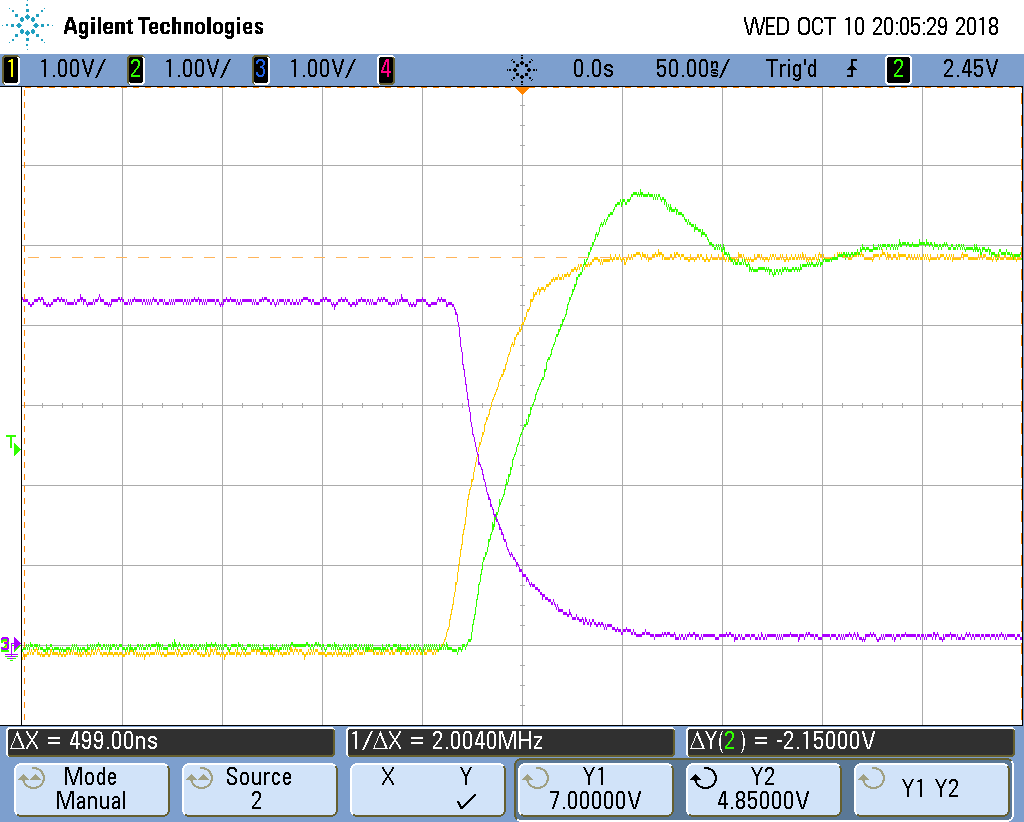
\includegraphics[width=6cm]{ejercicio2/OSC_LS_HC.png}
		\caption{LS alimentando al HC}
  	\end{center}
  \caption{Circuito utilizado}
  \label{7_fig1}
  \end{minipage}
  \begin{minipage}[b]{0.4\textwidth}
    \begin{center}
  		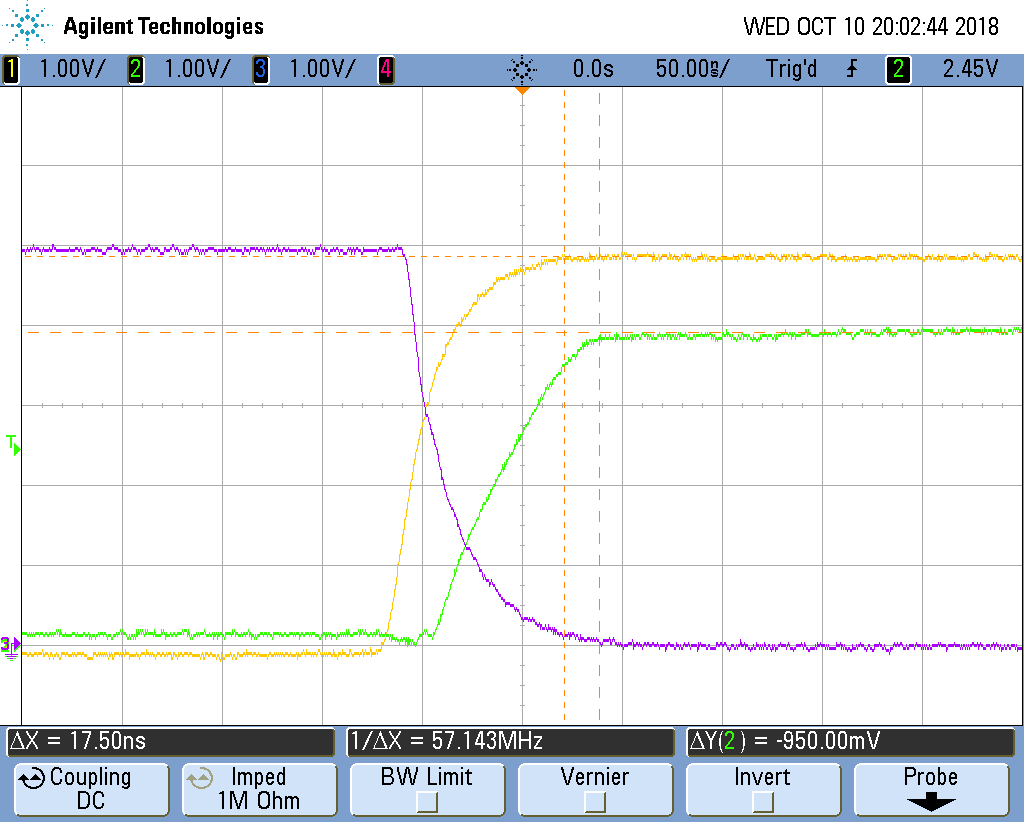
\includegraphics[width=6cm]{ejercicio2/OSC_HC_LS.png}
		\caption{HC alimentando al LS}
	\end{center}
  \caption{Implementaci\'on con 74HC112}
  \label{7_fig2}
 \end{minipage}
\end{center}
\end{figure}

\begin{figure}[hbtp]
	\centering
		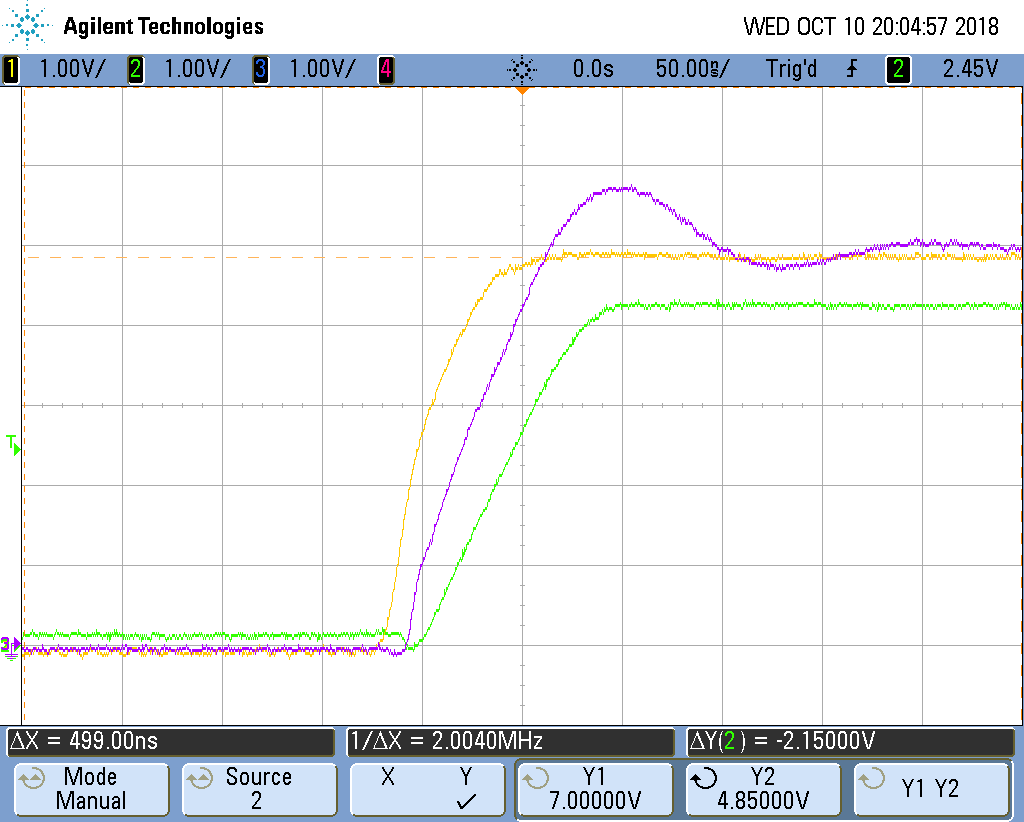
\includegraphics[width=8cm]{ejercicio2/OSC_AMBAS.png}
	\caption{Ambas señales sobrepuestas}
\end{figure}

En las im\'agenes anteriores la señal amarilla es la de entrada, la cual corresponde a una onda cuadrada que va de 0V a 5V. La señal verde es la de salida y la violeta es la señal intermedia (la señal que esta entre compuerta y compuerta). Mientras que en la tercer im\'agen est\'an sobrepuestas ambas señales de salida, donde la amarilla corresponde a la de entrada, la señal verde a la salida del 74LS02 y la señal violeta es la salida del 74HC02.




\part*{Ejercicio 3}

Se nos solicitó simplificar e implementar la siguiente tabla de verdad, y analizar las consecuencias de utilizar una metodología de menor costo.


\begin{figure}[H]
\begin{center}
  \begin{minipage}[b]{0.4\textwidth}
  	\begin{center}
  		\begin{tabular}{ccc|c}
A & B & C & Y \\ 
\hline
0 & 0 & 0 & 0 \\  
0 & 0 & 1 & 1 \\  
0 & 1 & 0 & 1 \\  
0 & 1 & 1 & 1 \\  
1 & 0 & 0 & 0 \\  
1 & 0 & 1 & 1 \\  
1 & 1 & 0 & 0 \\  
1 & 1 & 1 & 0 \\  
\end{tabular} 
  	\end{center}
  \caption{Tabla de verdad dada} 
  \label{3_fig1}
  \end{minipage}
  \begin{minipage}[b]{0.4\textwidth}
    \begin{center}
  		\begin{Karnaughvuit}
   \minterms{1,2,3,5}
   \maxterms{0,4,6,7}
   \indeterminats{}
   \implicant{1}{5}{green}
   \implicant{3}{2}{blue}
\end{Karnaughvuit}
	\end{center}
  \caption{Mapa de Karnaugh} 
  \label{3_fig2}
 \end{minipage}
\end{center}
\end{figure}

%\begin{center}
%\begin{tabular}{ccc|c}
%A & B & C & Y \\ 
%\hline
%0 & 0 & 0 & 0 \\  
%0 & 0 & 1 & 1 \\  
%0 & 1 & 0 & 1 \\  
%0 & 1 & 1 & 1 \\  
%1 & 0 & 0 & 0 \\  
%1 & 0 & 1 & 1 \\  
%1 & 1 & 0 & 0 \\  
%1 & 1 & 1 & 0 \\  
%\end{tabular} 
%\end{center}

%\begin{center}
%\begin{Karnaughvuit}
%   \minterms{1,2,3,5}
%   \maxterms{0,4,6,7}
%   \indeterminats{}
%   \implicant{1}{5}{green}
%   \implicant{3}{2}{blue}
%\end{Karnaughvuit}
%\end{center}

%\[Y = \bar{B}C + \bar{A}B \]
%\[Y = \overline{\overline{\bar{B}C + \bar{A}B}} \]
%\[Y = \overline{\overline{(\bar{B}C)}.\overline{(\bar{A}B)}} \]

%\begin{wrapfigure}{l}{4.5cm}
%\begin{center}
%\[Y = \bar{B}C + \bar{A}B \]
%\[Y = \overline{\overline{\bar{B}C + \bar{A}B}} \]
%\[Y = \overline{\overline{(\bar{B}C)}.\overline{(\bar{A}B)}} \]
%\caption{Función Lógica}
%\label{3_fig6}
%\end{center}
%\end{wrapfigure}

\newcommand{\mybox}
{%
    \begin{wrapfigure}{o}{0.3\textwidth}
\begin{center}
\[Y = \bar{B}C + \bar{A}B \]
\[Y = \overline{\overline{\bar{B}C + \bar{A}B}} \]
\[Y = \overline{\overline{(\bar{B}C)}.\overline{(\bar{A}B)}} \]
\caption{Función Lógica}
\label{3_fig6}
\end{center}
    \end{wrapfigure}\par\noindent
}

\mybox%

Expresada la función lógica en esta forma, se puede realizar una implementación de menor costo utilizando solamente dos integrados, un integrado con compuertas NAND y uno con compuertas NOT. El diagrama del circuito logico resultante se muestra en la Figura \ref{3_fig3}

%\begin{figure}[H]
%\begin{center}
%%\begin{circuitikz}[scale=1]
\draw
(0,0) node[nand port](nand1){}
(0,3) node[nand port](nand2){}
(3,1.5) node[nand port](nand3){}
(nand1.in 1) ++(left:4) node(A){}
(nand1.in 2) ++(left:4)++(down:1) node(B1){}

(nand2.in 1) ++(left:4) node[left](B2){}
(nand2.in 2) ++(left:4)++(down:1) node(C){}

(B2) ++(right:2) node[american not port](not2){}
(A) ++(right:2) node[american not port](not1){}

(B2) to[short,o-](not2.in) (not2.out) -- (nand2.in 1)
(C) to[short,o-] ++(right:3) |- (nand2.in 2)
(A) to[short,o-] (not1.in) (not1.out) -- (nand1.in 1)
(B1) to[short,o-] ++(right:3) |- (nand1.in 2)

(nand1.out) -- ++(right:0.5) |- (nand3.in 2)
(nand2.out) -- ++(right:0.5) |- (nand3.in 1)

(A) node[left](inA){A}
(B1) node[left](inB1){B}
(B2) node[left](inB2){B}
(C) node[left](inC){C}

(nand3.out) to[short,-o] ++(right:1) node[right](Y){Y}

;
\end{circuitikz}
%\resizebox{.5\linewidth}{!}{\parbox{\linewidth}{\begin{circuitikz}[scale=1]
\draw
(0,0) node[nand port](nand1){}
(0,3) node[nand port](nand2){}
(3,1.5) node[nand port](nand3){}
(nand1.in 1) ++(left:4) node(A){}
(nand1.in 2) ++(left:4)++(down:1) node(B1){}

(nand2.in 1) ++(left:4) node[left](B2){}
(nand2.in 2) ++(left:4)++(down:1) node(C){}

(B2) ++(right:2) node[american not port](not2){}
(A) ++(right:2) node[american not port](not1){}

(B2) to[short,o-](not2.in) (not2.out) -- (nand2.in 1)
(C) to[short,o-] ++(right:3) |- (nand2.in 2)
(A) to[short,o-] (not1.in) (not1.out) -- (nand1.in 1)
(B1) to[short,o-] ++(right:3) |- (nand1.in 2)

(nand1.out) -- ++(right:0.5) |- (nand3.in 2)
(nand2.out) -- ++(right:0.5) |- (nand3.in 1)

(A) node[left](inA){A}
(B1) node[left](inB1){B}
(B2) node[left](inB2){B}
(C) node[left](inC){C}

(nand3.out) to[short,-o] ++(right:1) node[right](Y){Y}

;
\end{circuitikz}}}
%\caption{Diagrama del circuito implementado} \label{3_fig3}
%\end{center}
%\end{figure}

%\begin{wrapfigure}{r}{6.5cm}
%\begin{center}
%\resizebox{.5\linewidth}{!}{\parbox{\linewidth}{\begin{circuitikz}[scale=1]
\draw
(0,0) node[nand port](nand1){}
(0,3) node[nand port](nand2){}
(3,1.5) node[nand port](nand3){}
(nand1.in 1) ++(left:4) node(A){}
(nand1.in 2) ++(left:4)++(down:1) node(B1){}

(nand2.in 1) ++(left:4) node[left](B2){}
(nand2.in 2) ++(left:4)++(down:1) node(C){}

(B2) ++(right:2) node[american not port](not2){}
(A) ++(right:2) node[american not port](not1){}

(B2) to[short,o-](not2.in) (not2.out) -- (nand2.in 1)
(C) to[short,o-] ++(right:3) |- (nand2.in 2)
(A) to[short,o-] (not1.in) (not1.out) -- (nand1.in 1)
(B1) to[short,o-] ++(right:3) |- (nand1.in 2)

(nand1.out) -- ++(right:0.5) |- (nand3.in 2)
(nand2.out) -- ++(right:0.5) |- (nand3.in 1)

(A) node[left](inA){A}
(B1) node[left](inB1){B}
(B2) node[left](inB2){B}
(C) node[left](inC){C}

(nand3.out) to[short,-o] ++(right:1) node[right](Y){Y}

;
\end{circuitikz}}}
%\caption{Diagrama del circuito implementado} 
%\label{3_fig3}
%\end{center}
%\end{wrapfigure}

\newcommand{\myboxi}
{%
    \begin{wrapfigure}{o}{0.3\textwidth}
\begin{center}
\resizebox{.5\linewidth}{!}{\parbox{\linewidth}{\begin{circuitikz}[scale=1]
\draw
(0,0) node[nand port](nand1){}
(0,3) node[nand port](nand2){}
(3,1.5) node[nand port](nand3){}
(nand1.in 1) ++(left:4) node(A){}
(nand1.in 2) ++(left:4)++(down:1) node(B1){}

(nand2.in 1) ++(left:4) node[left](B2){}
(nand2.in 2) ++(left:4)++(down:1) node(C){}

(B2) ++(right:2) node[american not port](not2){}
(A) ++(right:2) node[american not port](not1){}

(B2) to[short,o-](not2.in) (not2.out) -- (nand2.in 1)
(C) to[short,o-] ++(right:3) |- (nand2.in 2)
(A) to[short,o-] (not1.in) (not1.out) -- (nand1.in 1)
(B1) to[short,o-] ++(right:3) |- (nand1.in 2)

(nand1.out) -- ++(right:0.5) |- (nand3.in 2)
(nand2.out) -- ++(right:0.5) |- (nand3.in 1)

(A) node[left](inA){A}
(B1) node[left](inB1){B}
(B2) node[left](inB2){B}
(C) node[left](inC){C}

(nand3.out) to[short,-o] ++(right:1) node[right](Y){Y}

;
\end{circuitikz}}}
\caption{Diagrama del circuito implementado} 
\label{3_fig3}
\end{center}
    \end{wrapfigure}\par\noindent
}

\myboxi
El circuito implementado presenta una dificultad al transicionar entre miniterminos no adyacentes, pues no se pueden conmutar las entradas simultáneamente, entonces cuando uno esperaría ver en la salida un valor alto constante, observa una transición alto-bajo-alto. Si bien este pulso bajo que se observa es de muy corta duración, es suficiente para producir comportamientos inesperados en un eventual circuito lógico conectado a la salida de nuestra implementación. 

%\newpage

Las señales de alimentación se togglearon entre el mintermino 3 y 5 con el siguiente código utilizando una placa experimental Arduino UNO;

\lstinputlisting[language=C, frame=single]{ejercicio3/codigo.ino}

%\begin{figure}[H]
%\begin{center}
%\lstinputlisting[language=C, frame=single]{ejercicio3/codigo.ino}
%\end{center}
%\end{figure}

Como se comentó anteriormente en cada transición del mintermino 3 al 5, se pasa por el mintermino 7, al cual le corresponde un 0 en la tabla de verdad, mientras que en el pasaje del mintermino 5 al 3, se transiciona a través del mintermino 1, al cual le corresponde un 1 en la tabla de verdad. El pulso observado en la Figura \ref{3_fig4} corresponde al instante en que las entradas pasan por el mintermino 7.


%\begin{figure}[H]
%\begin{center}
%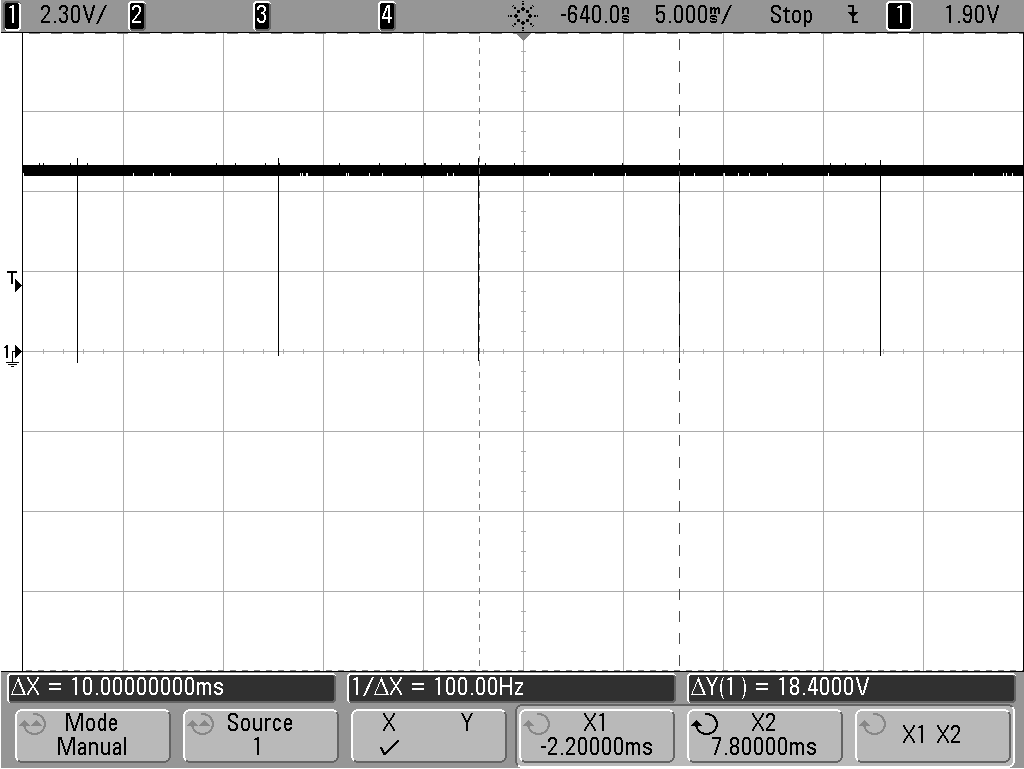
\includegraphics[scale=0.25]{ejercicio3/imagenes/riple.png}
%\caption{Respuesta a las transiciones mostradas} \label{3_fig2}
%\end{center}
%\end{figure}

\begin{figure}[H]
\begin{center}
  \begin{minipage}[b]{0.4\textwidth}
  	\begin{center}
  		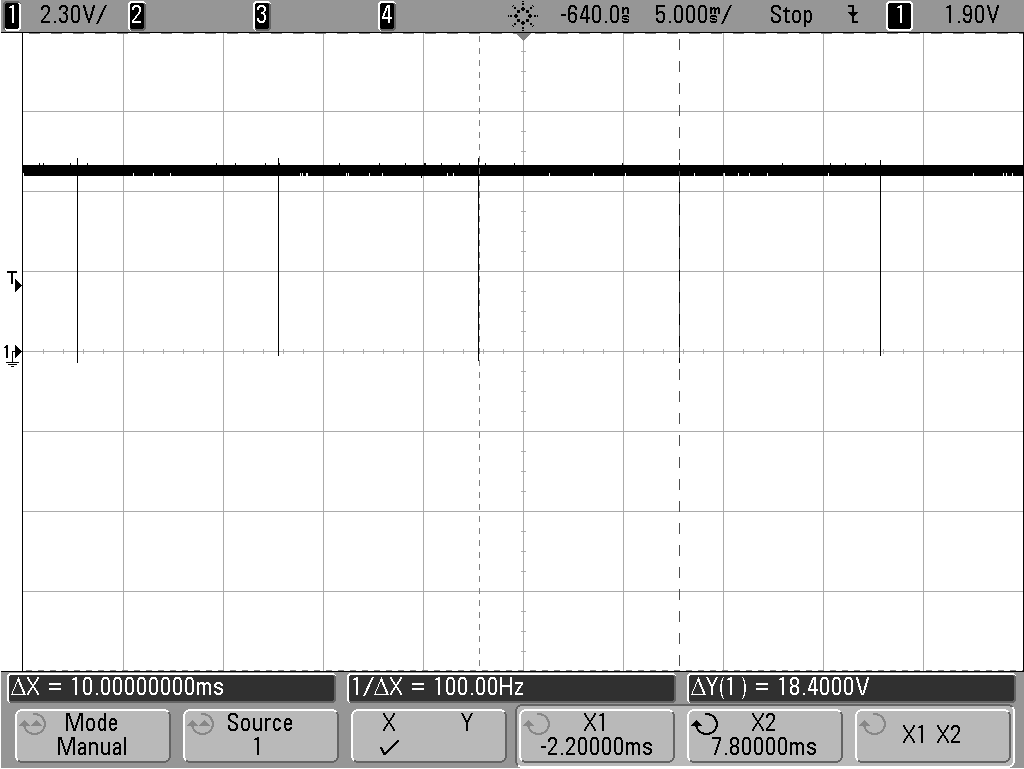
\includegraphics[scale=0.25]{ejercicio3/imagenes/riple.png}
  	\end{center}
  \caption{Respuesta a las transiciones mostradas} 
  \label{3_fig4}
  \end{minipage}
  \begin{minipage}[b]{0.4\textwidth}
    \begin{center}
  		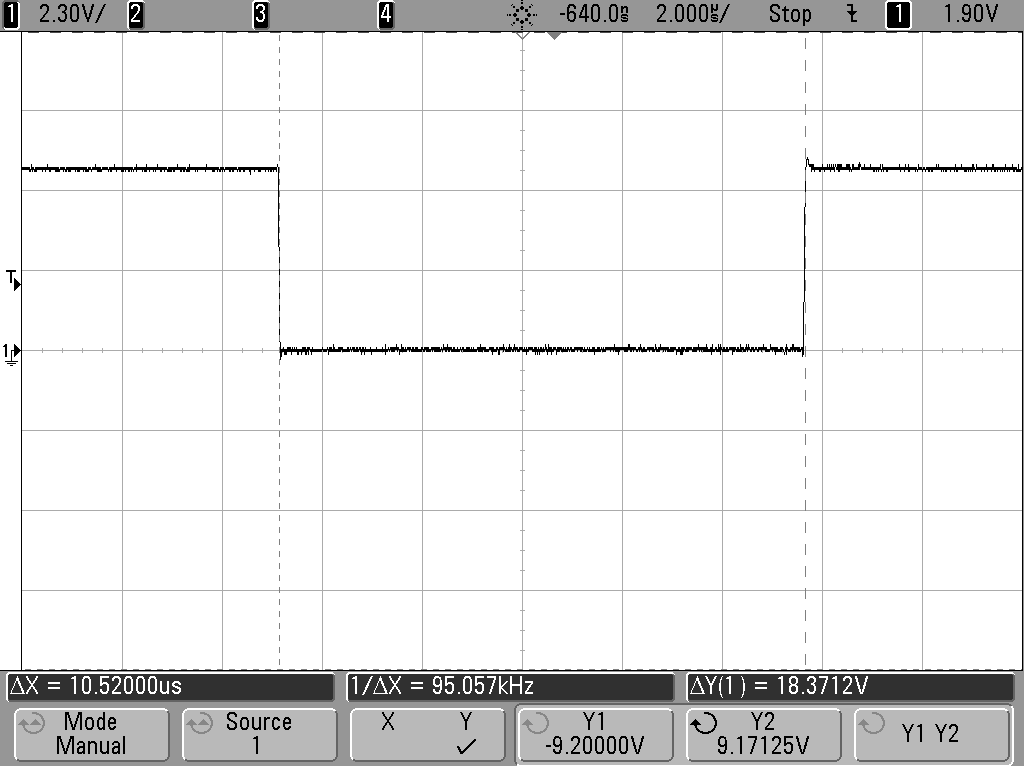
\includegraphics[scale=0.25]{ejercicio3/imagenes/tdown.png}
	\end{center}
  \caption{Ancho del pulso producido a la salida} 
  \label{3_fig5}
 \end{minipage}
\end{center}
\end{figure}

En la Figura \ref{3_fig5} se muestra una vista ampliada del pulso negativo que se mostró en la Figura \ref{3_fig4}. El ancho del pulso es de 10$\mu$seg, tiempo considerablemente largo como para producir cambios inesperados en circuitos posteriores, como ya se explicó.

%\begin{figure}[H]
%\begin{center}
%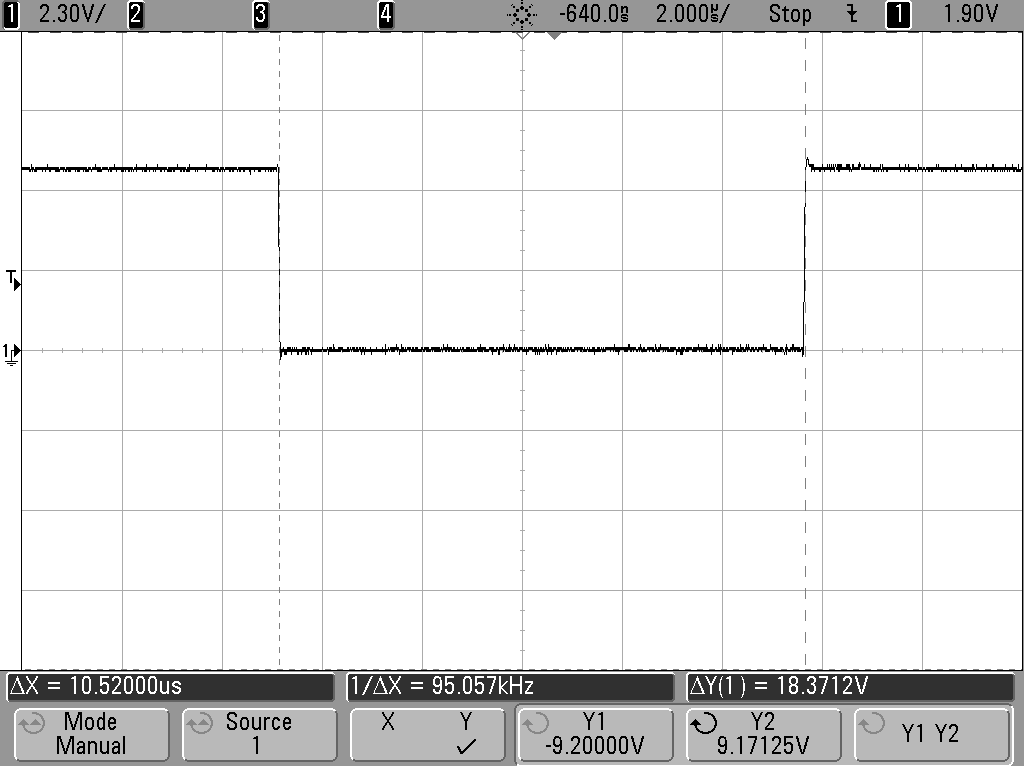
\includegraphics[scale=0.25]{ejercicio3/imagenes/tdown.png}
%\caption{Ancho del pulso producido a la salida} \label{3_fig3}
%\end{center}
%\end{figure}





Se nos solicitó medir los tiempos de propagación, rise time y fall time de una compuerta 74HC02 en vacío, y luego repetir el experimento implementando el circuito mostrado en la Figura \ref{4_fig3}. La compuerta NOR es una 74HC02 y las NAND son 74HC00.
%\begin{figure}[H]
%\centering
%\begin{circuitikz}[scale=1] \draw
(-1.4,0) to[short,*-o] (-2,0)
(0,0) node[nor port](myand1) {}
(myand1.in 1) -| (myand1.in 2)
(myand1.out) to[short] (0.5,0)
(2.5,3) node[nand port](nandgate1){}
(nandgate1.in 1) -| (nandgate1.in 2)
(2.5,1.5) node[nand port](nandgate2){}
(nandgate2.in 1) -| (nandgate2.in 2)
(2.5,0) node[nand port](nandgate3){}
(nandgate3.in 1) -| (nandgate3.in 2)
(2.5,-1.5) node[nand port](nandgate4){}
(nandgate4.in 1) -| (nandgate4.in 2)
(0.5,3) to[short,-] (0.5,-3)
(0.5,3)to[short,-*] (1.11,3)
(0.5,1.5) to[short,*-*] (1.11,1.5)
(0.5,0) to[short,*-*] (1.11,0)
(0.5,-1.5) to[short,*-*] (1.11,-1.5)
(nandgate1.out) -- (3,3)
to[R=1k] (4.5,3) to[empty led] (6.5,3)
(nandgate2.out) -- (3,1.5)
to[R=1k] (4.5,1.5) to[empty led,-*] (6.5,1.5)
(nandgate3.out) -- (3,0)
to[R=1k] (4.5,0) to[empty led,-*] (6.5,0)
(nandgate4.out) -- (3,-1.5)
to[R=1k] (4.5,-1.5) to[empty led,-*] (6.5,-1.5)
(0.5,-3) to[short] (3,-3)
to[R=560] (4.5,-3) to[empty led,-*] (6.5,-3)
(6.5,3) to[short] (6.5,-3.5)
(6.5,-3.5) node[ground]{}
;
\end{circuitikz}
%\caption{Circuito a implementar}
%\label{4_fig3} 
%\end{figure}

\begin{wrapfigure}{l}{6.5cm}
\begin{center}
\resizebox{.5\linewidth}{!}{\parbox{\linewidth}{\begin{circuitikz}[scale=1] \draw
(-1.4,0) to[short,*-o] (-2,0)
(0,0) node[nor port](myand1) {}
(myand1.in 1) -| (myand1.in 2)
(myand1.out) to[short] (0.5,0)
(2.5,3) node[nand port](nandgate1){}
(nandgate1.in 1) -| (nandgate1.in 2)
(2.5,1.5) node[nand port](nandgate2){}
(nandgate2.in 1) -| (nandgate2.in 2)
(2.5,0) node[nand port](nandgate3){}
(nandgate3.in 1) -| (nandgate3.in 2)
(2.5,-1.5) node[nand port](nandgate4){}
(nandgate4.in 1) -| (nandgate4.in 2)
(0.5,3) to[short,-] (0.5,-3)
(0.5,3)to[short,-*] (1.11,3)
(0.5,1.5) to[short,*-*] (1.11,1.5)
(0.5,0) to[short,*-*] (1.11,0)
(0.5,-1.5) to[short,*-*] (1.11,-1.5)
(nandgate1.out) -- (3,3)
to[R=1k] (4.5,3) to[empty led] (6.5,3)
(nandgate2.out) -- (3,1.5)
to[R=1k] (4.5,1.5) to[empty led,-*] (6.5,1.5)
(nandgate3.out) -- (3,0)
to[R=1k] (4.5,0) to[empty led,-*] (6.5,0)
(nandgate4.out) -- (3,-1.5)
to[R=1k] (4.5,-1.5) to[empty led,-*] (6.5,-1.5)
(0.5,-3) to[short] (3,-3)
to[R=560] (4.5,-3) to[empty led,-*] (6.5,-3)
(6.5,3) to[short] (6.5,-3.5)
(6.5,-3.5) node[ground]{}
;
\end{circuitikz}}}
\caption{Circuito a implementar}
\label{4_fig3}
\end{center}
\end{wrapfigure}

A continuación se nos solicitó aumentar la frecuencia del generador de señales a 100kHz y medir la tensión de alimentación, y repetir la experiencia conectando capacitores de desacople en los terminales de alimentación de los integrados.
Los resultados obtenidos para los tiempos de propagación, rise time y fall time de la compuerta 74HC02 en vacío fueron:

\begin{figure}[H]
\begin{flushright}
\begin{tabular}{|c|c|}
\hline 
Tiempo de propagación & 9.39 nseg \\ 
\hline 
Rise time & 9.93 nseg \\ 
\hline 
Fall time & 35.5 nseg \\ 
\hline 
\end{tabular}
\end{flushright}
\end{figure}

Cuando se implementó el circuito mostrado en la Figura \ref{4_fig3}, los valores obtenidos fueron:

\begin{center}
\begin{tabular}{|c|c|}
\hline 
Tiempo de propagación & 12.7 nseg \\ 
\hline 
Rise time & 38.8 nseg \\ 
\hline 
Fall time & 32.9 nseg \\ 
\hline 
\end{tabular}
\end{center}

Se observa que el tiempo de propagación y el fall time se ven ligeramente afectados. No así el rise time, el cuál es aproximadamente 4 veces mayor cuando se carga la salida de la compuerta NOR con el circuito mostrado.

\bigskip
Seguidamente se aumentó la frecuencia del generador de señales a 100kHz y se midió la señal de alimentación. La Figura \ref{4_fig1} muestra unos pequeños sobrepicos que coinciden con los flancos de la señal de entrada. Estos sobrepicos se poducen porque cuando las compuertas conmutan producen una demanda de corriente significativa, la cual es provista por la fuente de alimentación. La linea de alimentación de los integrados posee una impedancia despreciable cuando no hay variaciones de corriente en el circuito, sin embargo cuando conmutan las compuertas y las fluctuaciones en la corriente son repentinas, los efectos de la impedancia se manifiestan, y aparecen sobrepicos de tension en la linea.
%\begin{figure}[H]
%\centering
%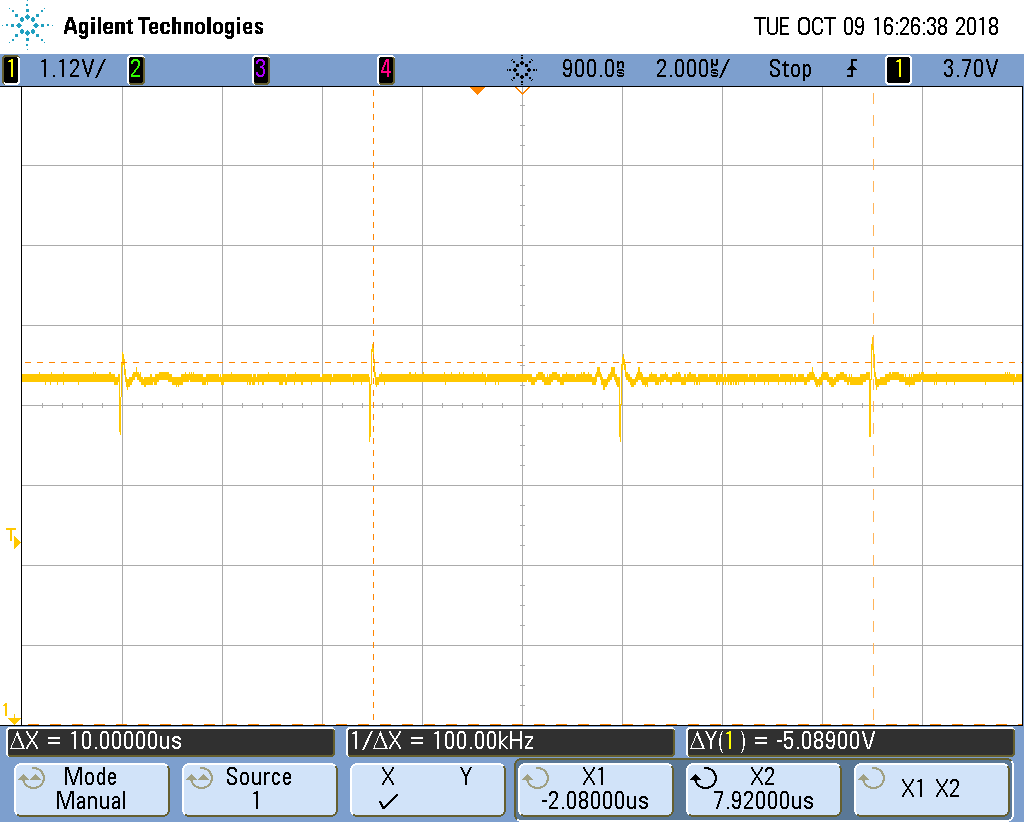
\includegraphics[scale=0.2]{imagenes/sin_capacitor.png}
%\caption{Tensión en el terminal de alimentacion del 74HC02 sin capacitor}
%\label{4_fig1} 
%\end{figure}

Para suavizar este efecto, se colocaron, como indica la consigna, capacitores de desacople en los terminales de alimentación de los circuitos integrados. Como muestra la Figura \ref{4_fig2}, el efecto es contrarrestado de forma significativa. De esta forma, cuando el circuito demanda un flujo de corriente repentinamente, el capacitor provee la corriente al integrado y no se producen cambios repentinos de corriente en la linea de alimentación.

%\begin{figure}[H]
%\centering
%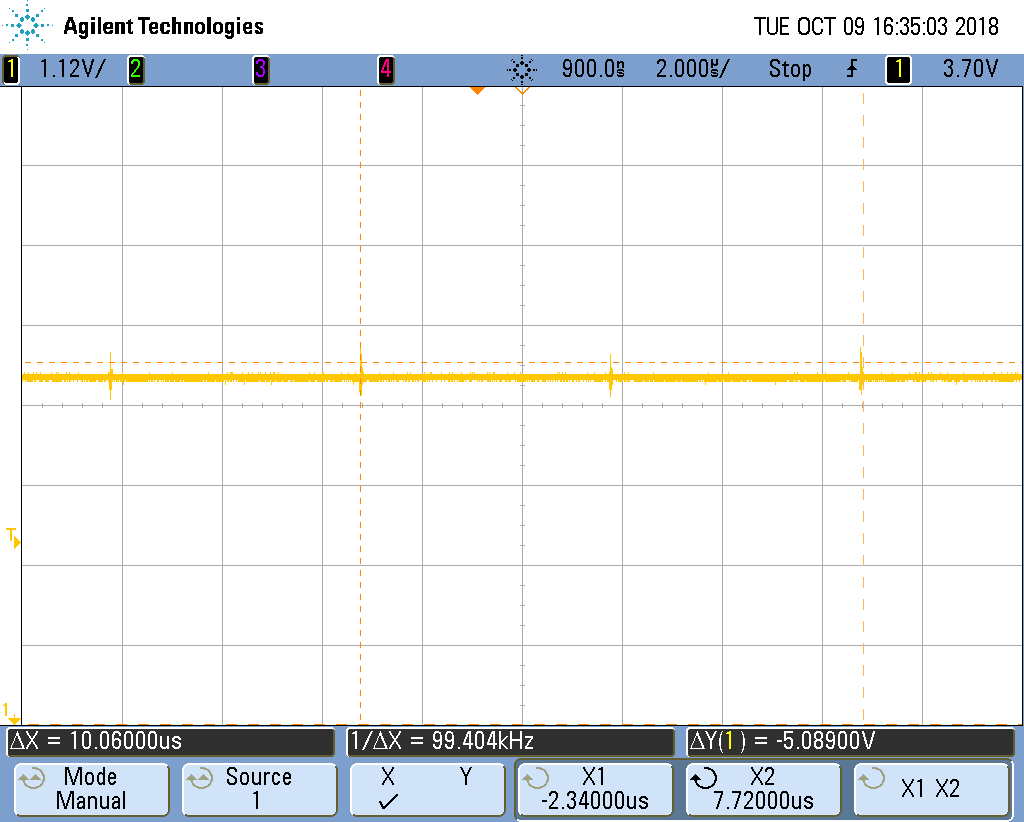
\includegraphics[scale=0.2]{imagenes/con_capacitor.png}
%\caption{Tensión en el terminal de alimentacion del 74HC02 con capacitor}
%\label{4_fig2} 
%\end{figure}

\begin{figure}[H]
\begin{center}
  \begin{minipage}[b]{0.4\textwidth}
  	\begin{center}
  		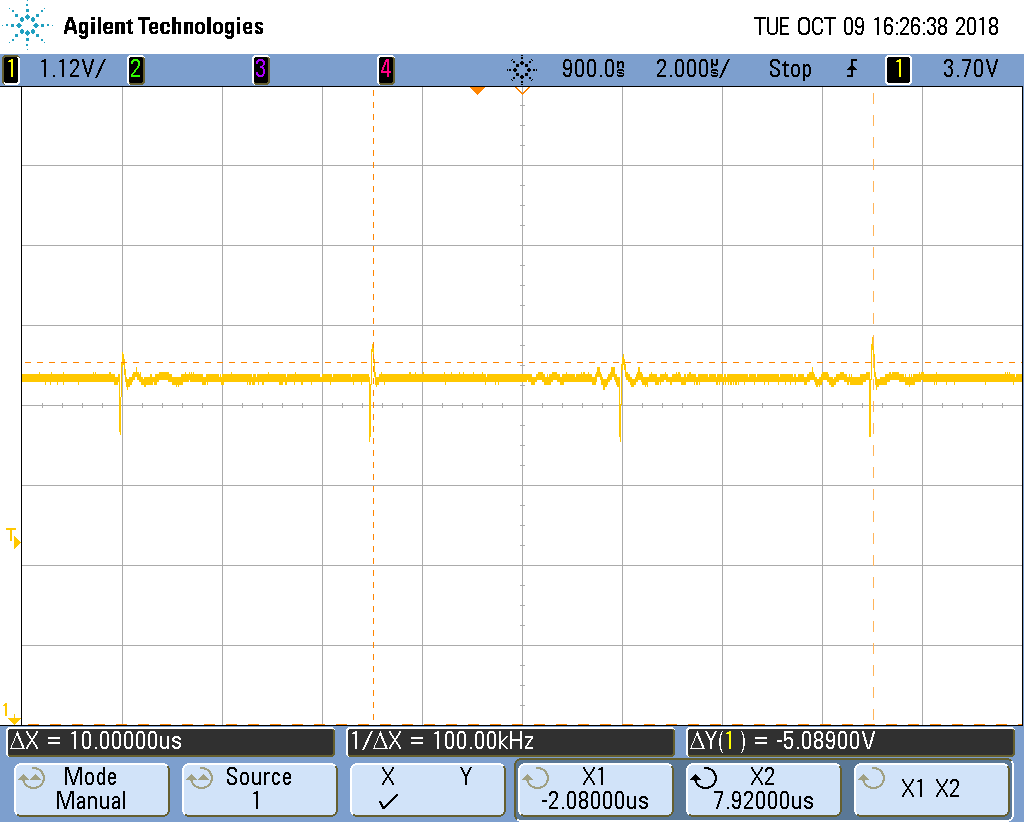
\includegraphics[scale=0.18]{imagenes/sin_capacitor.png}
  	\end{center}
  \caption{Tensión en el terminal de alimentacion del 74HC02 sin capacitor}
  \label{4_fig1} 
  \end{minipage}
  \begin{minipage}[b]{0.4\textwidth}
    \begin{center}
  		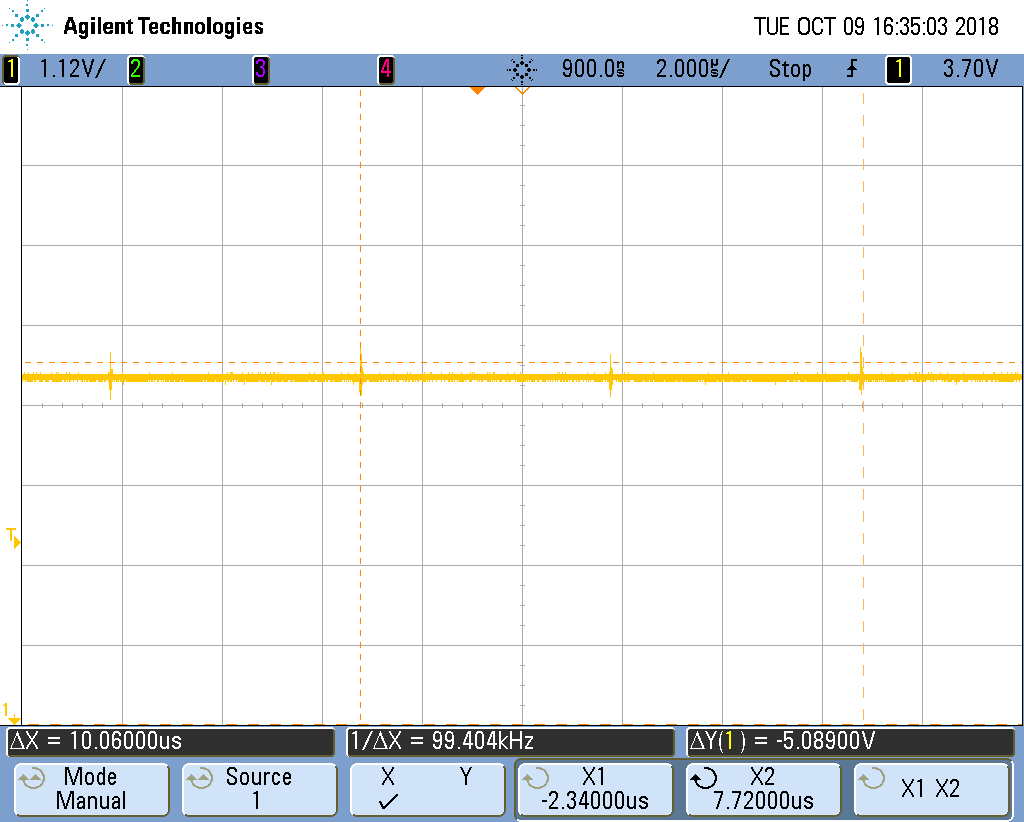
\includegraphics[scale=0.18]{imagenes/con_capacitor.png}
	\end{center}
  \caption{Tensión en el terminal de alimentacion del 74HC02 con capacitor}
  \label{4_fig2}
 \end{minipage}
\end{center}
\end{figure}








Alimentamos una compuerta AND de tecnolog\'ia TTL, integrado HD74LS08, conectando una entrada a la tensi\'on Vcc y la otra al generador de funciones. Tambi\'en alimentamos una compuerta OR de tecnolog\'ia CMOS, integrado SN74HC32N, conectando una entrada a tierra y la otra al generador de funciones. La alimentaci\'ion de ambos integrados es de 6V, el m\'aximo sugerido por ambos fabricantes. Analizando la salida podemos notar que la compuerta OR devuelve un pico de tensi\'on como ya notamos en la tecnolog\'ia CMOS y la compuerta AND devuelve solo 3,5V a la salida, ambos par\'ametros est\'an dentro de lo normal seg\'un las hojas de datos de cada una. Luego procedimos a conectar las compuertas de la siguiente forma:

\begin{figure}[hbtp]
\centering
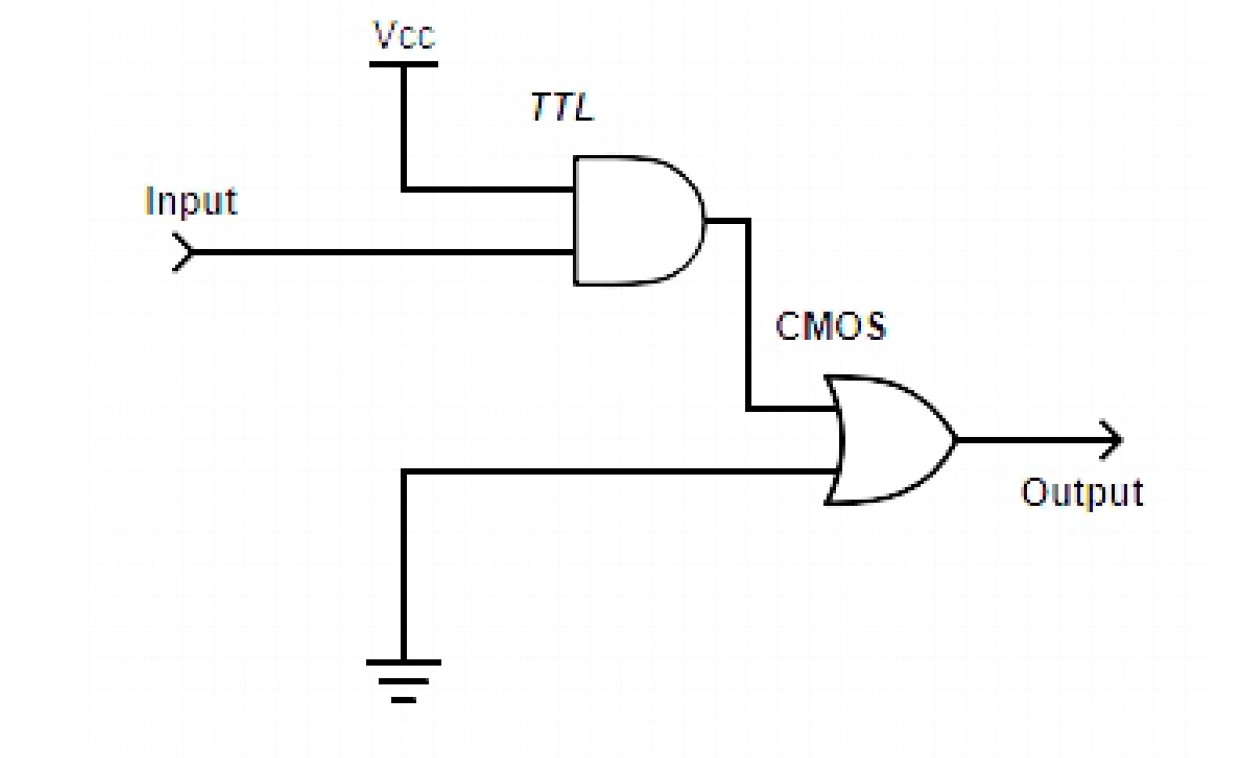
\includegraphics[width=8cm]{ejercicio5/E3_CirEj5.jpg}  
\caption{Circuito ejercicio 5}
\end{figure}


Midiendo en la salida de la OR esperar\'iamos que no hubiera salida o si la hubiera tuviera problemas, ya que la entrada m\'inima que acepta la OR es de 4,2V con la alimentaci\'on elegida y la AND otorga como ya mencionamos 3,5V. En nuestro caso el circuito l\'ogico funcion\'o como si no hubiera ning\'un tipo de problema, creemos que esto puede deberse a que las hojas de datos otorgan datos donde el fabricante se asegura que sus componentes funcionen pero pueden haber algunos que funcionen fuera del alcance determinado por el fabricante, esto quiere decir que puede funcionar pero no esta garantizado el buen funcionamiento. En caso de haber tenido alg\'un error hubi\'eramos optado por utilizar dos transistores para poner un pull-up que se active con la baja salida de la AND y alimente con $V_dd=5V$ la entrada de la OR como en el siguiente esquema.

\begin{figure}[hbtp]
\centering
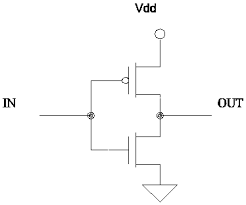
\includegraphics[width=5cm]{ejercicio5/PullUp.jpg} 
\caption{Circuito de Pull-Up}
\end{figure}



Se nos pidió implementar un Flip-Flop D y un Latch SR a partir de compuertas lógicas discretas, medir sus parámetros que consideramos importantes para la caracterización de su funcionamiento y comparar con equivalentes comerciales. Para verificar las tablas características de funcionamiento de los dispositivos se utilizó una placa experimental Arduino UNO para programar las distintas configuraciones de señales de entrada, y se midieron señales de entrada y salida en un osciloscopio digital. 

\subsection*{Latch SR}

%\begin{figure}[H]
%\centering
%\begin{circuitikz}[scale=1] \draw
(0,0) node[nand port](nandR){}
(0,4) node[nand port](nandS){}
(3,0.28) node[nand port](nandR2){}
++(right:0.7) node(nodo_Q){}
(nandR2.out) to[short, -o] ++(right:2) node[right]{$\bar{Q}$}
(3,3.72) node[nand port](nandS2){}
++(right:0.7) node(nodoQ){}
(nandS2.out) to[short, -o] ++(right:2) node[right]{Q}
(nandR.out) -| (nandR2.in 2)
(nandS.out) -| (nandS2.in 1)
(nandR2.in 1) to[short] ++(-0.5,0) to[short] ++(0,0.7) to[short] ++(2.5,1.5) coordinate(r)
(nandS2.in 2) to[short] ++(-0.5,0) to[short] ++(0,-0.7) to[short] ++(2.5,-1.5) coordinate(s)
(s) to[short,-*] (s|-nodo_Q)
(r) to[short,-*] (s|-nodoQ)

(nandS.in 2) to[short] ++(left:0.5) coordinate (s2)
(nandR.in 1) to[short] ++(left:0.5) coordinate (r2)
(r2) to[short] (r2|-s2)
(-3,2) coordinate (clk)
(clk) node[left](){Clk}
(clk) to[short, o-*] (clk-|s2)
(nandS.in 1) to[short, -o] (nandS.in 1-|clk) node[left](){S}
(nandR.in 2) to[short, -o] (nandR.in 2-|clk) node[left](){R}
;
\end{circuitikz}
%\caption{Latch SR implementado} \label{6_fig1}
%\end{figure}

%\begin{wrapfigure}{l}{6.5cm}
%\begin{center}
%\resizebox{.5\linewidth}{!}{\parbox{\linewidth}{\begin{circuitikz}[scale=1] \draw
(0,0) node[nand port](nandR){}
(0,4) node[nand port](nandS){}
(3,0.28) node[nand port](nandR2){}
++(right:0.7) node(nodo_Q){}
(nandR2.out) to[short, -o] ++(right:2) node[right]{$\bar{Q}$}
(3,3.72) node[nand port](nandS2){}
++(right:0.7) node(nodoQ){}
(nandS2.out) to[short, -o] ++(right:2) node[right]{Q}
(nandR.out) -| (nandR2.in 2)
(nandS.out) -| (nandS2.in 1)
(nandR2.in 1) to[short] ++(-0.5,0) to[short] ++(0,0.7) to[short] ++(2.5,1.5) coordinate(r)
(nandS2.in 2) to[short] ++(-0.5,0) to[short] ++(0,-0.7) to[short] ++(2.5,-1.5) coordinate(s)
(s) to[short,-*] (s|-nodo_Q)
(r) to[short,-*] (s|-nodoQ)

(nandS.in 2) to[short] ++(left:0.5) coordinate (s2)
(nandR.in 1) to[short] ++(left:0.5) coordinate (r2)
(r2) to[short] (r2|-s2)
(-3,2) coordinate (clk)
(clk) node[left](){Clk}
(clk) to[short, o-*] (clk-|s2)
(nandS.in 1) to[short, -o] (nandS.in 1-|clk) node[left](){S}
(nandR.in 2) to[short, -o] (nandR.in 2-|clk) node[left](){R}
;
\end{circuitikz}}}
%\caption{Latch SR implementado} 
%\label{6_fig1}
%\end{center}
%\end{wrapfigure}

\newcommand{\myboxa}
{%
    \begin{wrapfigure}{o}{0.3\textwidth}
\begin{center}
\resizebox{.5\linewidth}{!}{\parbox{\linewidth}{\begin{circuitikz}[scale=1] \draw
(0,0) node[nand port](nandR){}
(0,4) node[nand port](nandS){}
(3,0.28) node[nand port](nandR2){}
++(right:0.7) node(nodo_Q){}
(nandR2.out) to[short, -o] ++(right:2) node[right]{$\bar{Q}$}
(3,3.72) node[nand port](nandS2){}
++(right:0.7) node(nodoQ){}
(nandS2.out) to[short, -o] ++(right:2) node[right]{Q}
(nandR.out) -| (nandR2.in 2)
(nandS.out) -| (nandS2.in 1)
(nandR2.in 1) to[short] ++(-0.5,0) to[short] ++(0,0.7) to[short] ++(2.5,1.5) coordinate(r)
(nandS2.in 2) to[short] ++(-0.5,0) to[short] ++(0,-0.7) to[short] ++(2.5,-1.5) coordinate(s)
(s) to[short,-*] (s|-nodo_Q)
(r) to[short,-*] (s|-nodoQ)

(nandS.in 2) to[short] ++(left:0.5) coordinate (s2)
(nandR.in 1) to[short] ++(left:0.5) coordinate (r2)
(r2) to[short] (r2|-s2)
(-3,2) coordinate (clk)
(clk) node[left](){Clk}
(clk) to[short, o-*] (clk-|s2)
(nandS.in 1) to[short, -o] (nandS.in 1-|clk) node[left](){S}
(nandR.in 2) to[short, -o] (nandR.in 2-|clk) node[left](){R}
;
\end{circuitikz}}}
\caption{Latch SR implementado} 
\label{6_fig1}
\end{center}
    \end{wrapfigure}\par\noindent
}

\myboxa

Para la implementación del Latch SR se siguió el diseño del \emph{Gated SR Latch}, encontrado en la sección 5.2 de \emph{Fundamentals of Digital Logic with Verilog Design}, el mismo se muestra en la Figura \ref{6_fig1}. El dispositivo se implemetó utilizando compuertas NAND 74HC00, de tecnología CMOS.

Se analizó su correcto funcionamiento para las distintas configuraciones de señales de entrada, y se obtuvo la siguiente tabla característica:

\begin{center}
\begin{tabular}{ccc|c}
Clk & S & R & Q(t+1) \\ 
\hline 
0 & x & x & Q(t) \\ 
1 & 0 & 0 & Q(t) \\ 
1 & 1 & 0 & 1 \\ 
1 & 0 & 1 & 0 \\ 
1 & 1 & 1 & ? \\
\end{tabular} 
\end{center}

\begin{figure}[H]
\begin{center}
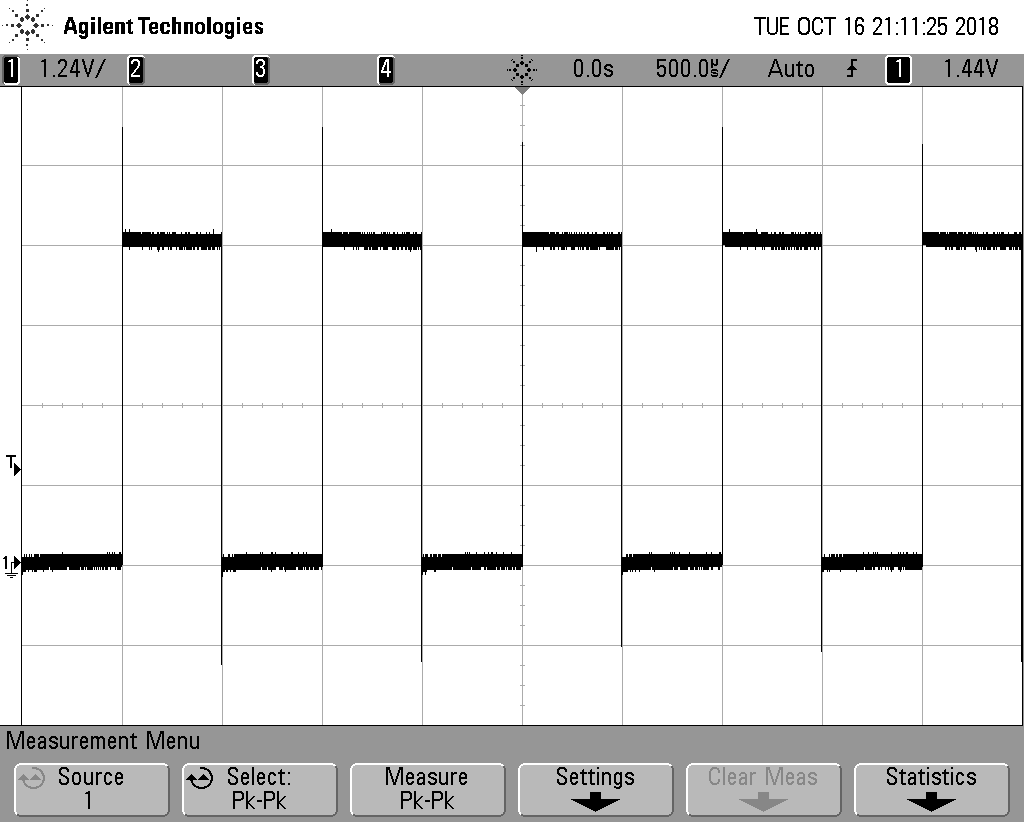
\includegraphics[scale=0.15]{ejercicio6/sr_1.png}
\caption{Estado inestable del Latch SR} \label{6_fig4}
\end{center}
\end{figure}

Las respuestas obtenidas para las distintas configuraciones coinciden con los valores teóricos esperados. Sin embargo, como lo indica el análisis del circuito, la configuración de señales de entrada $Clk=1$, $S=1$ y $R=1$ presenta una inestabilidad, en la cual el valor de salida $Q(t=1)$ no se establece en ningún valor. Para esta configuración, se registró en la Figura \ref{6_fig4} la forma de la salida.

En cuanto a los tiempos de respuesta de la compuerta, se midieron los tiempos de rise, fall y propagación, obteniendose los siguientes valores:

\begin{center}
\begin{tabular}{|c|c|}
\hline 
Rise Time & 27.6 nseg \\ 
\hline 
Fall Time & 26.8 nseg \\ 
\hline 
Propagación & 12.7 nseg \\ 
\hline 
\end{tabular} 
\end{center}

Se buscaron integrados comerciales de tecnología CMOS que implementen un Latch SR para comparar los parámetros medidos. El integrado CD4043 hallado es un integrado 3-state, motivo por el cual, quizás, difieran sus parámetros de los nuestros. Los tiempos de respuesta presentes en la hoja de datos del CD4043 son:

\begin{center}
\begin{tabular}{|c|c|}
\hline 
Rise Time & 100 nseg \\ 
\hline 
Fall Time & 100 nseg \\ 
\hline 
Propagación & 150 nseg \\ 
\hline 
\end{tabular} 
\end{center}


\subsection*{Flip-Flop D}
Para la implementación del Flip-Flop D, se siguió al igual que para el Latch SR el diseño presentado en la sección 5.3 y 5.4 de \emph{Fundamentals of Digital Logic with Verilog Design}. Se utilizó la configuración de dos Latch D master-slave, para lograr un Flip-Flop D activado por flanco ascendente. 

\begin{figure}[H]
\centering
\resizebox{.5\linewidth}{!}{\parbox{\linewidth}{\begin{circuitikz}[scale=1] \draw
(0,0) node[nand port](nandR){}
(0,4) node[nand port](nandS){}
(3,0.28) node[nand port](nandR2){}
++(right:0.7) node(nodo_Q){}
(nandR2.out) to[short, -o] ++(right:2) node[right]{$\bar{Q}$}
(3,3.72) node[nand port](nandS2){}
++(right:0.7) node(nodoQ){}
(nandS2.out) to[short, -o] ++(right:2) node[right]{Q}
(nandR.out) -| (nandR2.in 2)
(nandS.out) -| (nandS2.in 1)
(nandR2.in 1) to[short] ++(-0.5,0) to[short] ++(0,0.7) to[short] ++(2.5,1.5) coordinate(r)
(nandS2.in 2) to[short] ++(-0.5,0) to[short] ++(0,-0.7) to[short] ++(2.5,-1.5) coordinate(s)
(s) to[short,-*] (s|-nodo_Q)
(r) to[short,-*] (s|-nodoQ)

(nandS.in 2) to[short] ++(left:0.5) coordinate (s2)
(nandR.in 1) to[short] ++(left:0.5) coordinate (r2)


(r2) to[short] (r2|-s2)
(-5,2) coordinate(clk)
(clk) node[left](){Clk}
(clk) to[short, o-*] (clk-|s2)
(nandS.in 1) to[short, -o] (nandS.in 1-|clk) node[left](nodoS){D}
(-3,-0.28) node[american not port](notS){}
(notS.out) to[short] (nandR.in 2)
(notS.in) to[short] ++(left:0.5) coordinate(notin)
(notin) to[short,-*] (notin|-nodoS)

;
\end{circuitikz}}}
\caption{Modulo Latch D} \label{6_fig2}
\end{figure}

En la Figura \ref{6_fig2} se muestra la implementación de un módulo Latch D, el cual se utilzará, como se explicó para implementar el Flip-Flop D, ilustrado en la Figura \ref{6_fig3}


\begin{figure}[H]
\centering
\resizebox{.5\linewidth}{!}{\parbox{\linewidth}{\begin{circuitikz}[scale=1] \draw
(0,0) node[draw,minimum width=2cm,minimum height=2.4cm,anchor=south west]{}
(5,0) node[draw,minimum width=2cm,minimum height=2.4cm,anchor=south west]{}

(0,0.6) node[right](Clkm){Clk}
(0,1.8) node[right](Dm){D}
(2,0.6) node[left](Qm_){$\bar{Q}$}
(2,1.8) node[left](Qm){Q}



(5,0.6) node[right](Clks){Clk}
(5,1.8) node[right](Ds){D}
(7,0.6) node[left](Qs_){$\bar{Q}$}
(7,1.8) node[left](Qs){Q}

;
\draw
[thick,dashed] (-2,-2.5) rectangle (8,3);

\draw
(0,1.8) to[short,-o] ++ (left:3) node[left](D){D}
(0,0.6) to[short,-o] ++ (left:3) node[left](clk){Clk}

(-1,0.6) to[short,*-] ++(down:2) to [short] ++(right:1) node(notin){}
++(right:1)node[american not port](not){}
(notin) to[short] (not.in)
(not.out) to[short] ++(right:2) node(notout){}
(notout) to[short,-] (notout|-Clks)
to[short] (5,0.6)

(2,1.8) to[short] (5,1.8)

(7,1.8) to[short,-o] ++(right:2) node[right](Q){Q}
(7,0.6) to[short,-o] ++(right:2) node[right](noQ){$\bar{Q}$}
;
\end{circuitikz}}}
\caption{Diagrama Flip-Flop D} \label{6_fig3}
\end{figure}

La respuesta de las salidas en función a las entradas fue la esperada, cumpliéndose la siguiente tabla característica de un Flip-Flop D de flanco ascendente:

\begin{center}
\begin{tabular}{cc|c}
Clk & D & Q(t+1) \\ 
\hline 
\texttiming[timing/c/rising arrows, timing/c/arrow pos=.7]{2{C}} & 0 & 0 \\ 
\texttiming[timing/c/rising arrows, timing/c/arrow pos=.7]{2{C}} & 1 & 1 \\ 
\texttiming[timing/c/falling arrows, timing/c/arrow pos=.7]{HC}  & x & Q(t) \\
\end{tabular} 
\end{center}

Se midieron los tiempos de rise, fall y de propagación. Se obtuvieron los siguientes resultados:


\begin{center}
\begin{tabular}{|c|c|}
\hline 
Tiempo de Propagación & 18.8 nseg \\ 
\hline 
Rise Time & 27.8 nseg \\ 
\hline 
Fall Time & 27.6 nseg \\ 
\hline 
\end{tabular} 
\end{center}

Los resultados obtenidos se contrastan con los datos provistos por la hoja de datos del integrado comercial 74HC74, que implementa un Flip-Flop D. Los tiempos de propagación y de transición que se especifican son:

\begin{center}
\begin{tabular}{|c|c|}
\hline 
Tiempo de Propagación & 17 nseg \\ 
\hline 
Tiempo de Transición & 7 nseg \\ 
\hline 
\end{tabular} 
\end{center}

La diferencia apreciada entre los tiempos de transición medidos y los especificados en la hoja de datos del integrado comercial, puede deberse a que los tiempos de transición de las señales provistas por el Arduino UNO son significativamente mayores a los tiempos de respuesta de las compuertas utilizadas para implementar el Flip Flop, por lo tanto esto induce un error en la medición. 

%Lo hecho con imagenes es temporal, tal vez provisiempre
\part*{Ejercicio 7}
%Se nos solicitó implementar mediante compuertas lógicas un contador asincrónico y otro sincrónico, ambos %de 3 bits y determinar la máxima velocidad de opeación de ambos.

\subsection*{Contador Asincr\'onico}
Para el contador asincr\'onico se sigui\'o el esquema mostrado en la Figura \ref{7_fig1}. Se implement\'o utilizando Flip-Flops JK mediante integrados 74HC112, como puede observarse en la Figura \ref{7_fig2}. Utilizamos una señal cuadrada otorgada por el generador de señales, de 5V con un ciclo de trabajo del 50\%. En particular nuestro contador va de 7 a 0, cuenta hacia atr\'as, trabaja con flancos descendentes del Clock para el bit menos significativo y con flancos ascendentes para los últimos 2 bits.

%\begin{figure}[H]
%\begin{center}
%
\includegraphics[scale=0.25]{ejercicio7/imagenes/asynccircuito.png}
%\caption{Circuito utilizado para el contador asincronico} \label{7_fig1}
%\end{center}
%\end{figure}

\begin{figure}[H]
\begin{center}
  \begin{minipage}[b]{0.4\textwidth}
  	\begin{center}
  		
\includegraphics[scale=0.25]{ejercicio7/imagenes/asynccircuito.png}
  	\end{center}
  \caption{Circuito utilizado}
  \label{7_fig1}
  \end{minipage}
  \begin{minipage}[b]{0.4\textwidth}
    \begin{center}
  		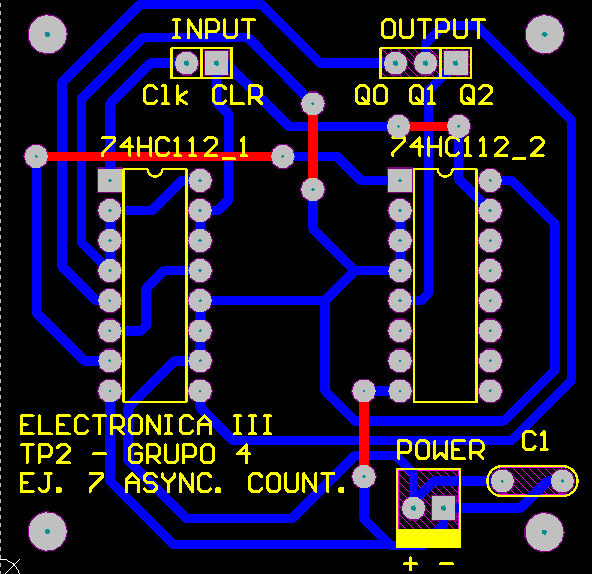
\includegraphics[scale=0.25]{ejercicio7/imagenes/asyncaltium.png}
	\end{center}
  \caption{Implementaci\'on con 74HC112}
  \label{7_fig2}
 \end{minipage}
\end{center}
\end{figure}


%Los flip-flops se conectan en cascada, donde se utiliza la salida $Q$ o $Q^{*}$ (dependiendo si queremos trabajar con flancos ascendentes o descendentes) conectada a la entrada clock de cada flip-flop después del primero. Al primero se conecta la señal deseada como Clock, nosotros utilizamos una señal cuadrada otorgada por el generador de señales, de 5V con un ciclo de trabajo del 50\%. En particular nuestro contador va de 7 a 0, cuenta hacia atr\'as, trabaja con flancos descendentes del Clock (cuando este pasa de valer 1 a 0) para el bit menos significativo y con flancos ascendentes para los últimos 2 bits( cuando el bit anterior pasa de 0 a 1) ya que los integrados 74HC112 tienen la entrada del clock negada y le conectamos $Q^{*}$, lo que equivale a conectar $Q$. Esto puede observarse junto a su correcto funcionamiento en la Figura \ref{7_fig3} donde si vamos desde arriba hacia abajo tenemos el Clock, $Q_0$ (bit menos significativo) ,$Q_1$ y $Q_2$.


%\begin{figure}[H]
%\begin{center}
%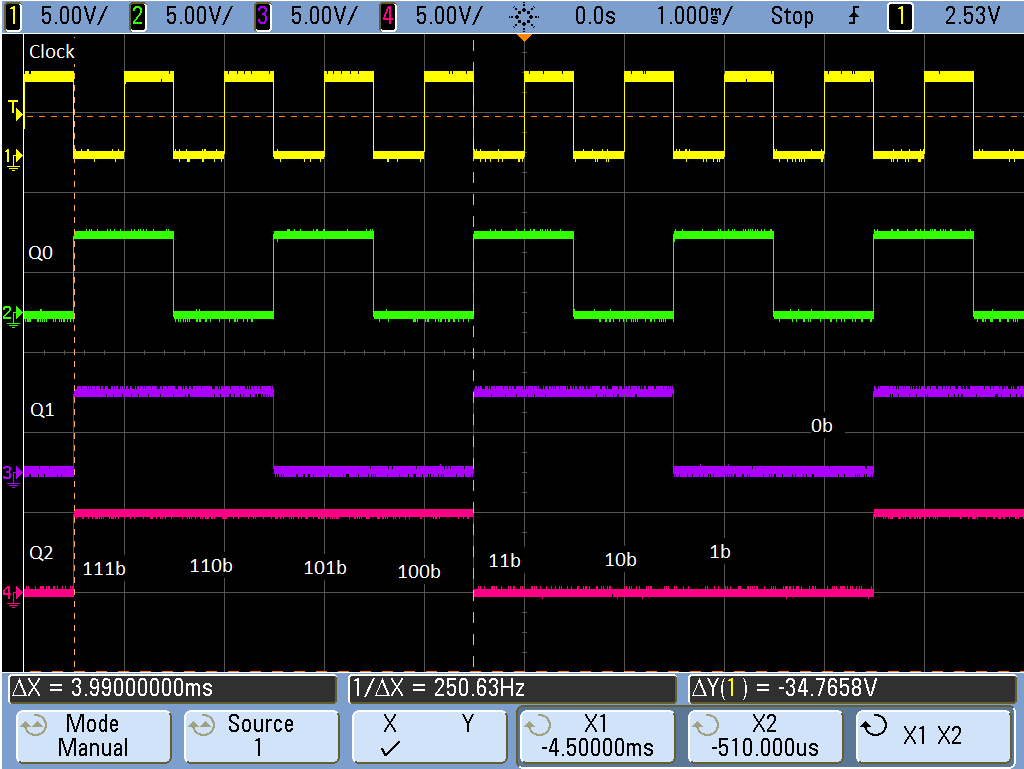
\includegraphics[scale=0.25,left]{ejercicio7/imagenes/async.png}
%\caption{Comportamiento del contador} \label{7_fig3}
%\end{center}
%\end{figure}

%\begin{wrapfigure}{l}{6.5cm}
%\begin{center}
%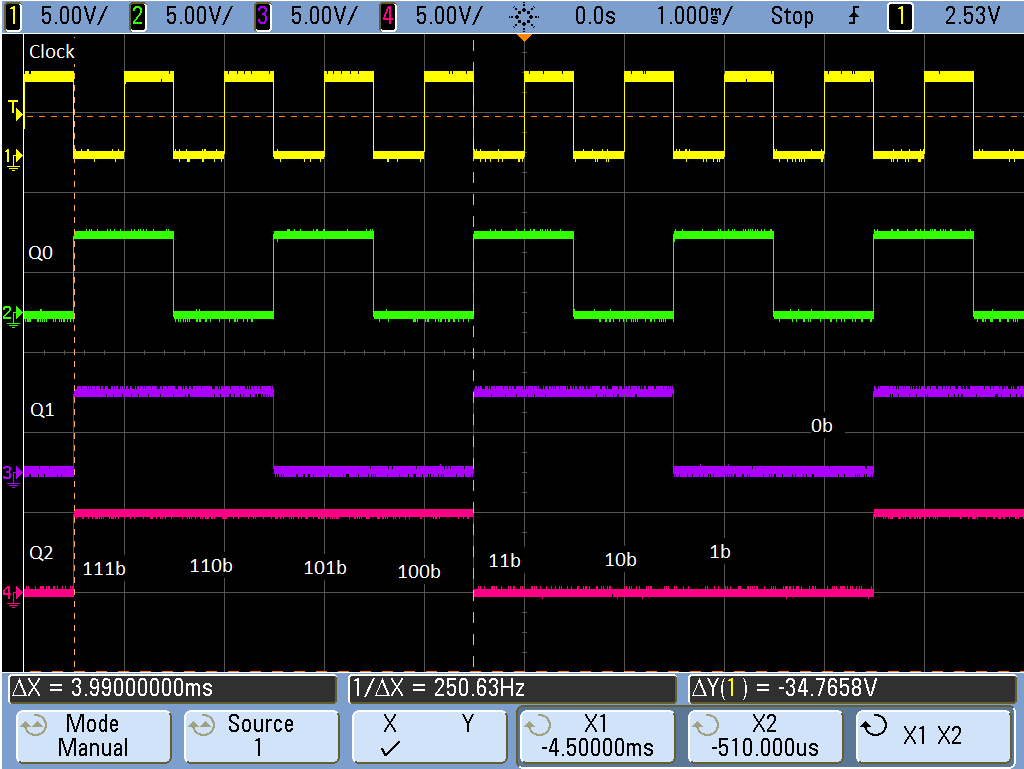
\includegraphics[scale=0.25,left]{ejercicio7/imagenes/async.png}
%\caption{Comportamiento del contador}\label{7_fig3}
%\end{center}
%\end{wrapfigure} 

%A modo de aclaración, podemos notar también en la Figura \ref{7_fig3} que mientras el bit menos significativo cambia con el flanco descendente del Clock, cuando este pasa de valer 1 a 0, los otros bits cambian cuando el bit anterior pasa de valer 0 a 1 ya que en nuestro caso la señal que le llega a cada entrada clock de los últimos dos flip-flops se encuentra conectada $Q^{*}$ pero las entradas clock de los integrados 74HC112 estan negadas, por lo que equivaldría a enviar la señal $Q$.

%En este tipo de contador, las salidas (que representan a los bits) no cambian exactamente al mismo
%En este tipo de contador 

\begin{wrapfigure}{l}{6.5cm}
\begin{center}
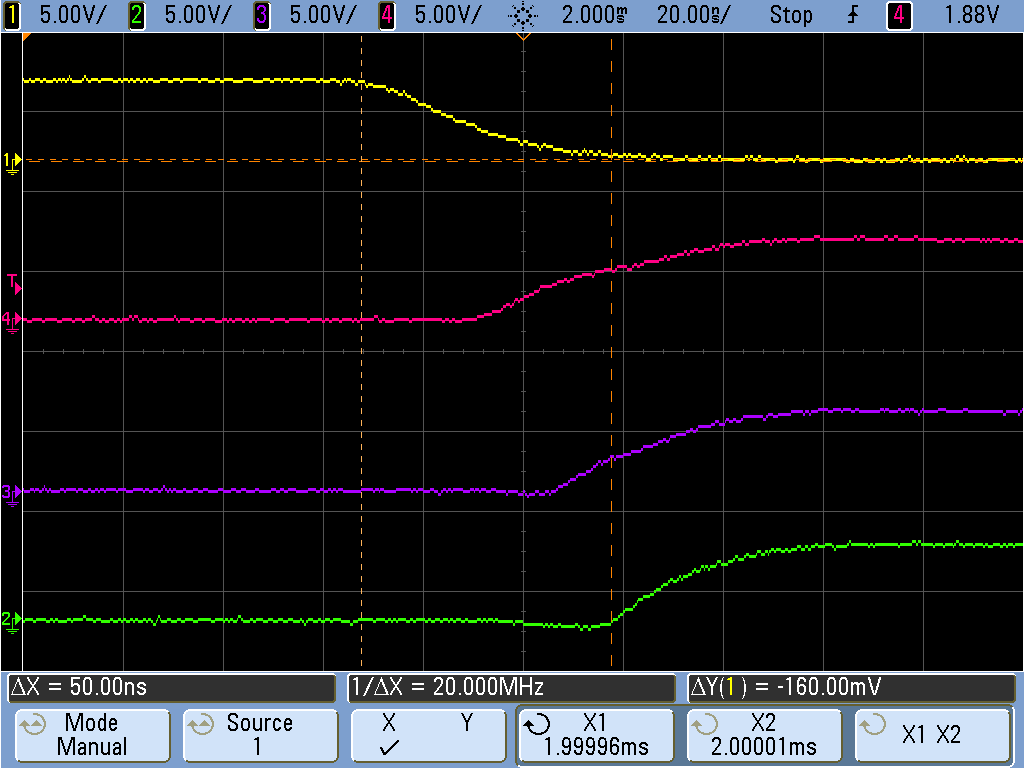
\includegraphics[scale=0.25]{ejercicio7/imagenes/timepropagation.png}
\caption{Medicion del delay acumulado}\label{7_fig3}
\end{center}
\end{wrapfigure}

Las salidas no cambian al mismo tiempo, hay un delay entre que la señal conectada a la entrada clock del flip-flop cambia hasta que la salida correspondiente también lo hace, entonces tenemos un delay total m\'as grande a mayor cantidad de flip-flops conectados en cascada, habr\'a un mayor retraso entre que la señal del clock cambia y lo hace el bit m\'as significativo. Esto es una desventaja de estos contadores porque hay que tener cuidado con la velocidad con la que trabaja el circuito ya que esta no puede superar la frecuencia que se obtiene luego de medir el m\'aximo delay acumulado por todas las compuertas, también sucede con estos contadores que pasamos por estados falsos hasta llegar a cambiar el bit m\'as significativo pero cambia tan r\'apido que esto no suele ser un problema grave para muchas aplicaciones.

Medimos el tiempo de propagaci\'on total desde que la señal del Clock comienza a descender hasta que el bit m\'as significativo ($Q_2$) comienza a elevarse y obtuvimos un valor de 50 ns (ver Figura \ref{7_fig3}), observamos el datasheet y el fabricante nos dice que trabajando a 5V y a 25 ºC el tiempo de propagaci\'on de cada flip-flop es de 17 ns, con las 3 compuertas tendríamos 51 ns por lo que comprobamos que lo medido es aproximado al valor te\'orico esperado. En las Figuras \ref{7_fig4},\ref{7_fig5},\ref{7_fig6},\ref{7_fig7} podemos ver el comportamiento del circuito a medida que aumentamos la frecuencia del Clock, a grandes frecuencias podemos ver como las señales medidas empiezan a tener un comportamiento extraño que puede deberse a que el ancho de banda del osciloscopio que utilizamos no era el suficiente y que este esta interviniendo en las mediciones, pero a grandes rasgos podemos notar que a pesar de todo se mantiene entre los valores que el integrado detecta como 1 y como 0 según sea el caso, pero al llegar a 23.8 MHz podemos ver que los valores de las salidas tooglean, varían entre 0 y 1 y esto se debe a que ya mi tiempo de delay es mayor al periodo de la señal con la que estoy trabajando, al mirar el datasheet observamos que el fabricante nos dice que en las condiciones que trabajamos no debemos de pasar los 70 MHz, y esto dividido entre los 3 flip-flops me da 23.33 MHz.

%esto acarrea otro problema el cual es que de esta manera no puedo pasar directamente de un número a otro, dependiendo el caso paso por más o menos estados falsos. Esto no es un problema para la mayoría de los casos ya que los cambios son muy rápidos, por lo que es tolerable para distintas aplicaciones.

%\begin{figure}[H]
%\begin{center}
%  \begin{minipage}[b]{0.4\textwidth}
%  	\begin{center}
%  		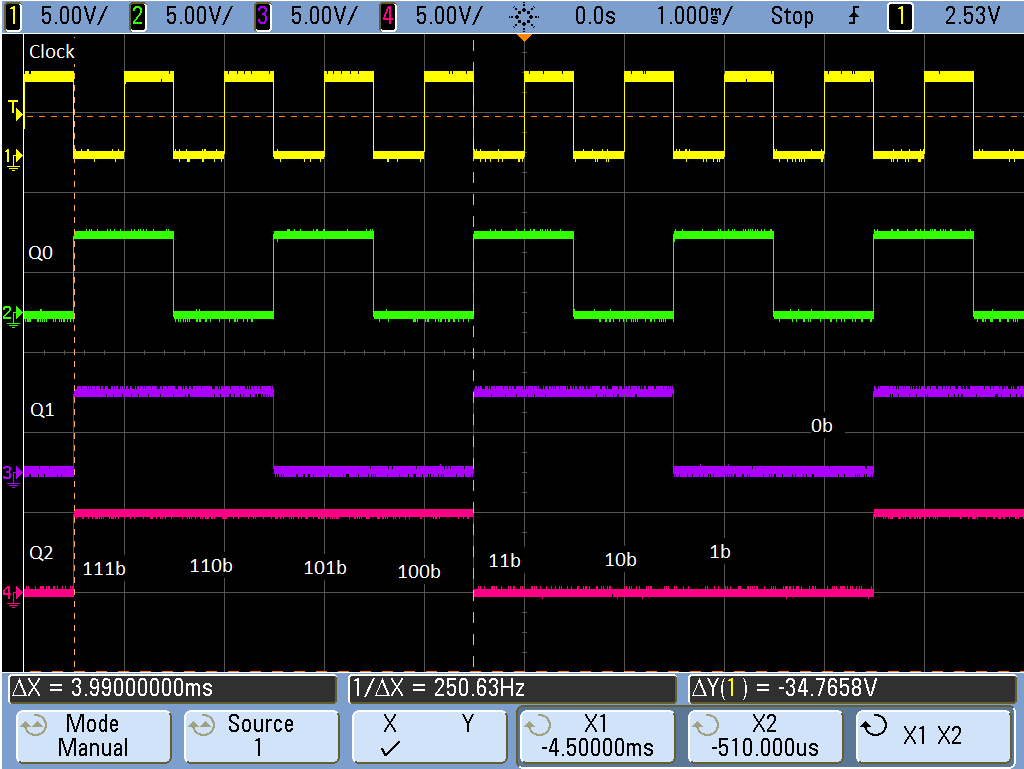
\includegraphics[scale=0.25]{ejercicio7/imagenes/async.png}
%  	\end{center}
%  \caption{Comportamiento del contador}
%  \label{7_fig3}
%  \end{minipage}
%  \begin{minipage}[b]{0.4\textwidth}
%    \begin{center}
%  		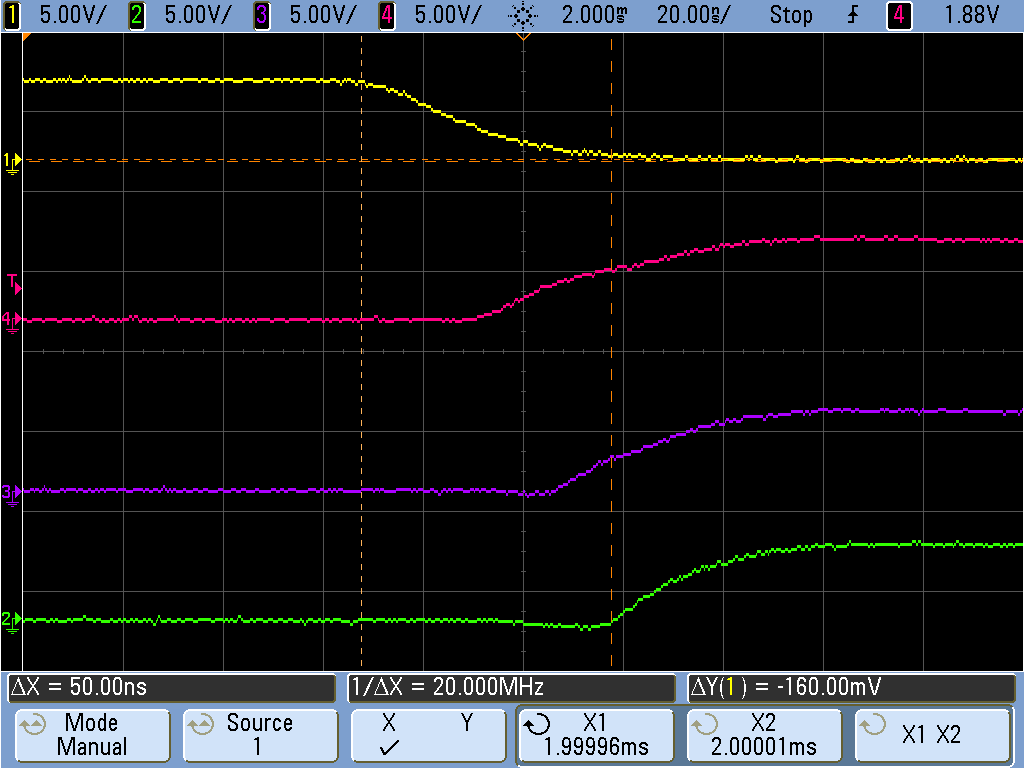
\includegraphics[scale=0.25]{ejercicio7/imagenes/timepropagation.png}
%	\end{center}
%  \caption{Medicion del delay acumulado}
%  \label{7_fig4}
% \end{minipage}
%\end{center}
%\end{figure}

\begin{figure}[H]
\begin{center}
  \begin{minipage}[b]{0.4\textwidth}
  	\begin{center}
  		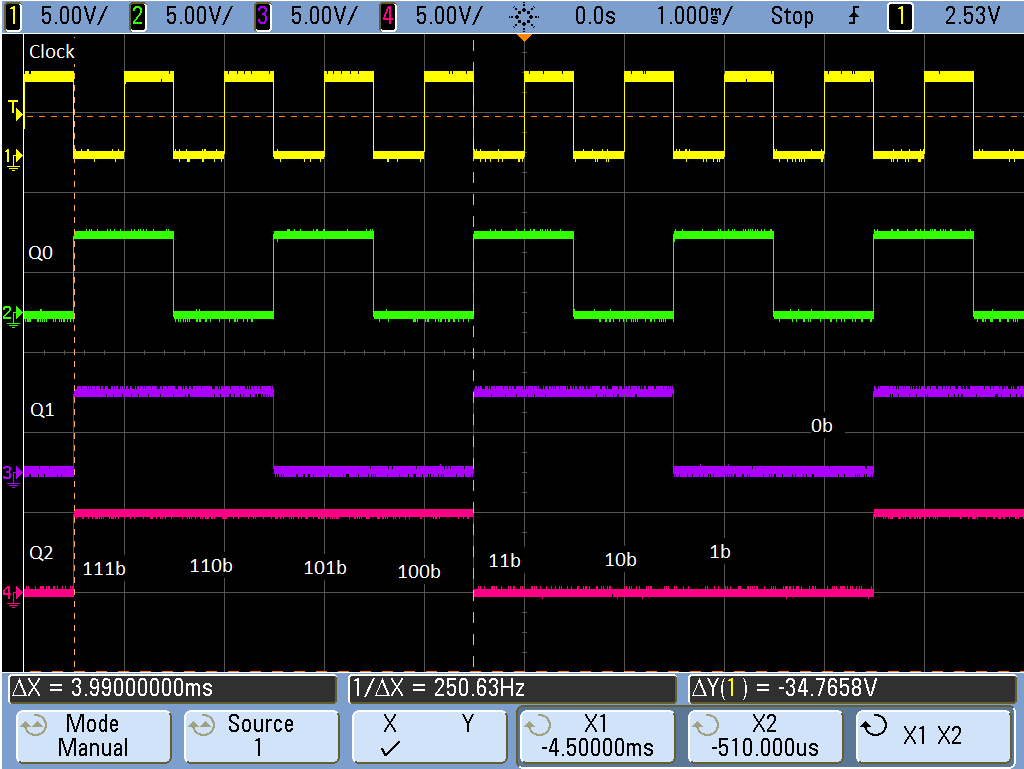
\includegraphics[scale=0.2]{ejercicio7/imagenes/async.png}
  	\end{center}
  \caption{Comportamiento a bajas frec}
  \label{7_fig4}
  \end{minipage}
  \begin{minipage}[b]{0.4\textwidth}
  	\begin{center}
  		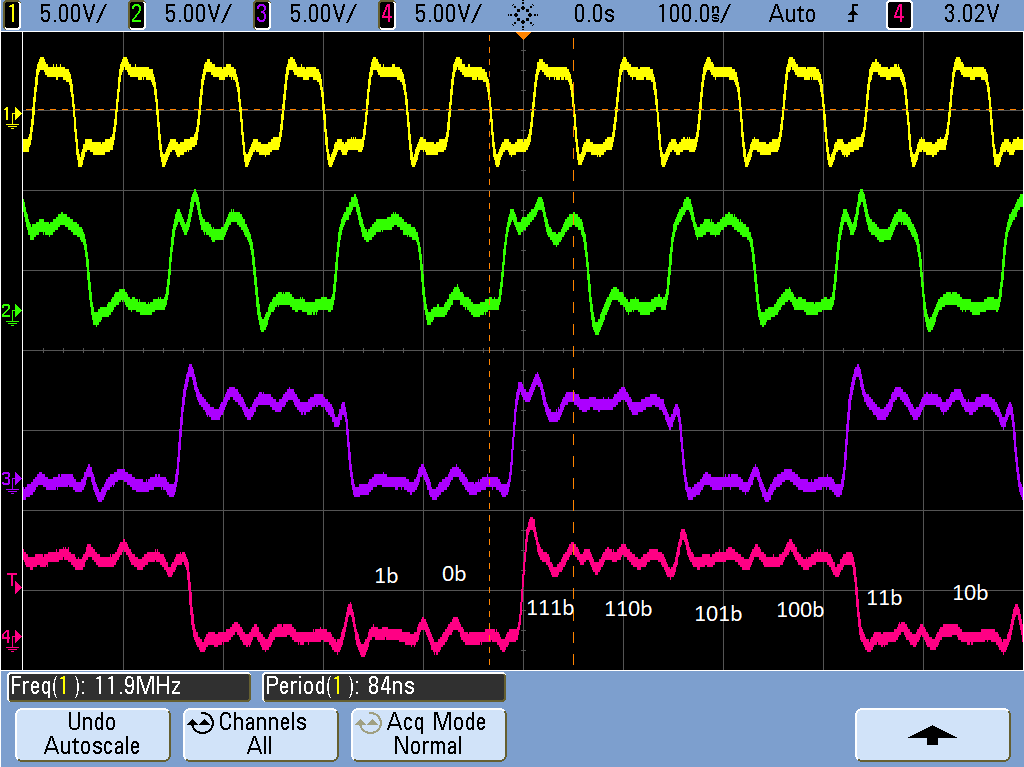
\includegraphics[scale=0.2]{ejercicio7/imagenes/async2.png}
  	\end{center}
  \caption{Comportamiento a 11.9 MHz}
  \label{7_fig5}
  \end{minipage}
  \begin{minipage}[b]{0.4\textwidth}
    \begin{center}
  		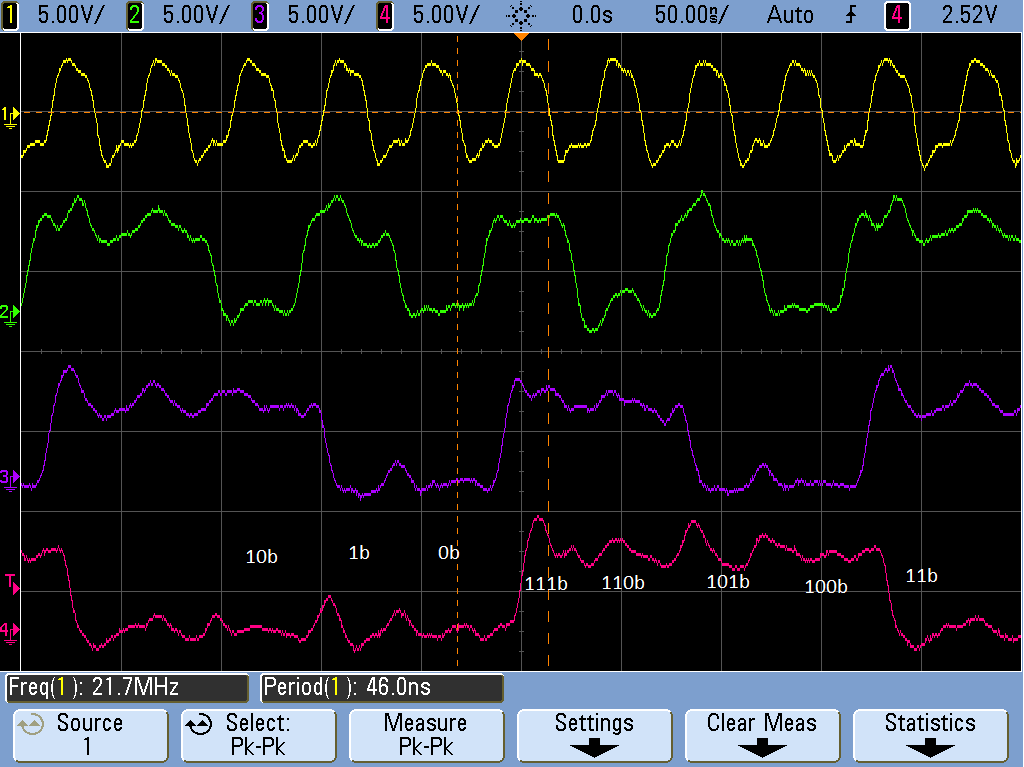
\includegraphics[scale=0.2]{ejercicio7/imagenes/async3.png}
	\end{center}
  \caption{A 21.7 MHz}
  \label{7_fig6}
 \end{minipage}
   \begin{minipage}[b]{0.4\textwidth}
    \begin{center}
  		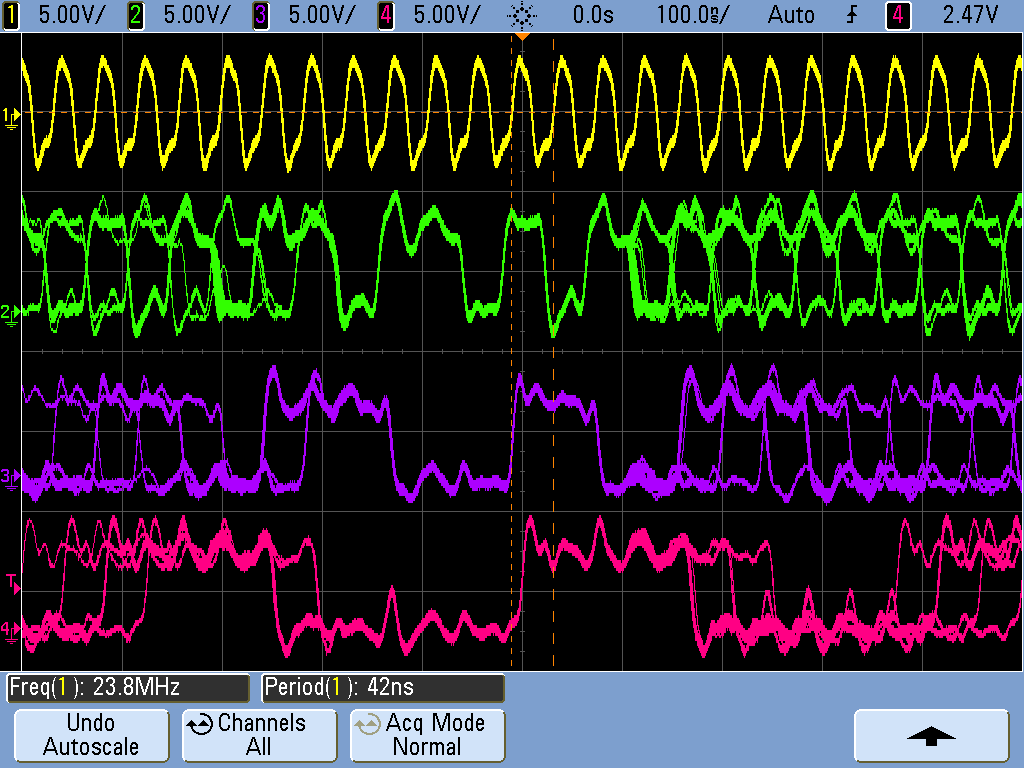
\includegraphics[scale=0.2]{ejercicio7/imagenes/async4.png}
	\end{center}
  \caption{A 23.8 MHz}
  \label{7_fig7}
 \end{minipage}
\end{center}
\end{figure}

%\begin{wrapfigure}{l}{6.5cm}
%\begin{center}
%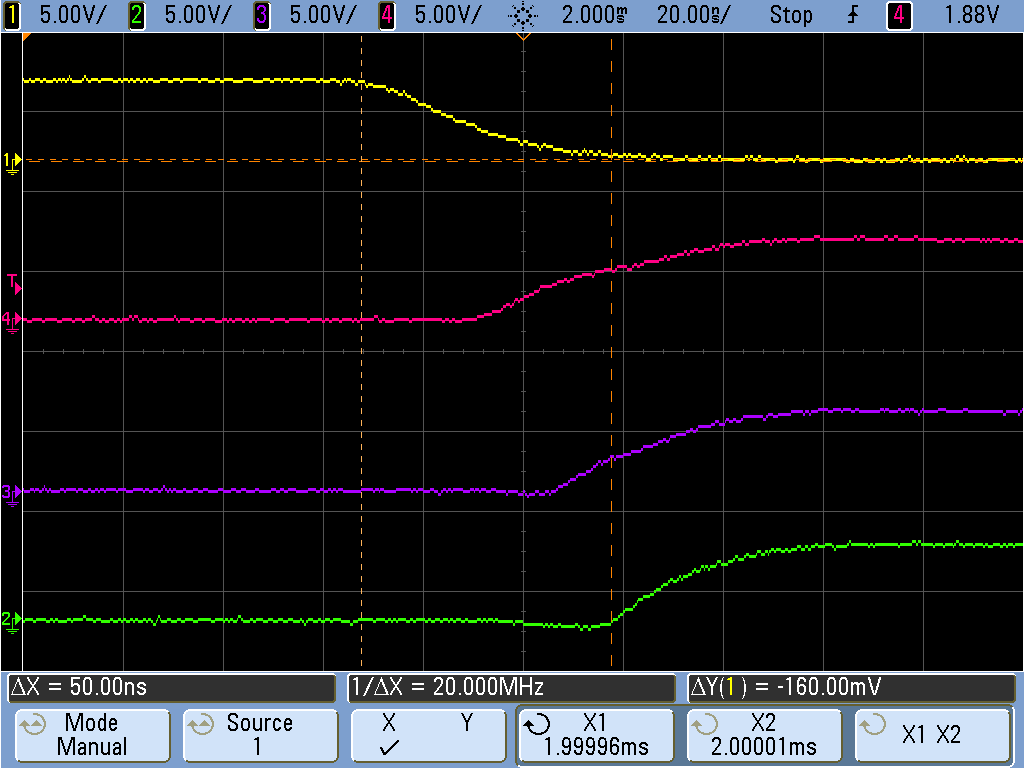
\includegraphics[scale=0.25,left]{ejercicio7/imagenes/timepropagation.png}
%\caption{Comportamiento del contador}\label{7_fig4}
%\end{center}
%\end{wrapfigure}
 


%\begin{figure}[H]
%\begin{center}
%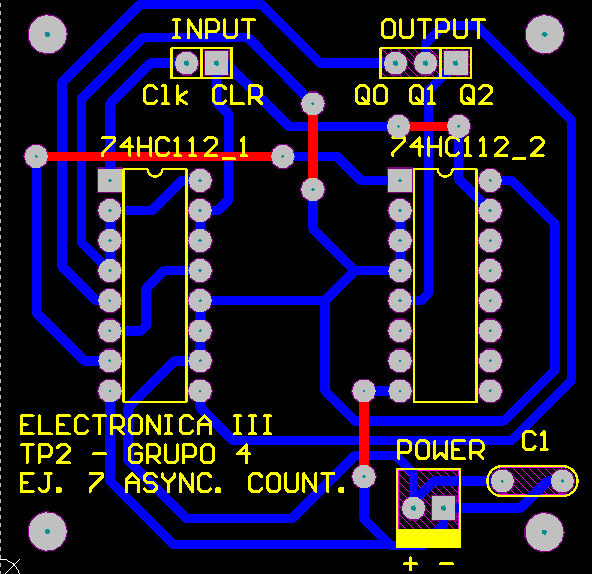
\includegraphics[scale=0.25]{ejercicio7/imagenes/asyncaltium.png}
%\caption{Implementación con 74HC112} \label{7_fig2}
%\end{center}
%\end{figure}

\subsection*{Contador Sincr\'onico}
Este contador que avanza de forma descendente al igual que el contador anterior, pero con la diferencia de que los clock de cada Flip-Flop estar\'an conectados directamente a la misma señal en lugar de usar la señal del flip-flop anterior. Este cambio har\'a que cada parte se active con el flanco derecho de la misma señal, reaccionando todas las partes del contador a un mismo tiempo determinado, siempre y cuando se trate del mismo componente o tengan las mismas caracter\'isticas temporales, y no obtener un arrastre en el delay final.
\newline
Al mirar el tiempo de propagaci\'on de este circuito obtenemos que solo hay 24ns de delay, 17ns correspondiente al flip-flop (ahora no se suman sus delay porque son independientes) y 7ns correspondientes a la compuerta AND del circuito, esto quiere decir que reci\'en a los 42,66MHz el circuito empezar\'a a togglear porque el tiempo de delay superar\'a la frecuencia de trabajo al igual que en el caso anterior. No pudimos obtener im\'agenes de este caso porque se necesita tener un osciloscopio de m\'as de 200MHz debido a que si el instrumento no tiene un ancho de banda 5 veces mayor a la frecuencia de trabajo se perder\'an detalles de la señal que impiden tener una medici\'on correcta.




\subsection*{Trigger HC-SR04}

El primer paso en el diseño del circuito fue implementar un bloque circuital que proporcione el pulso de trigger al sensor HC-SR04, el cuál, como indica en las especificaciones, debe ser de $10 \mu seg$, sin embargo, habiéndose realizado pruebas utilizando una placa de experimentación Arduino UNO, se determinó que se puede disparar el sensor con pulsos de ordenes superiores de extensión. Esta observación tiene relevancia, ya que generar un pulso tan breve mediante un pulsador mecánico trae ciertas complejidades. Dicho esto, a continuación se explica el circuito utilizado para generar el pulso.
\bigskip

\begin{figure}[H]
\begin{center}
\begin{circuitikz}[scale=1] \draw
(0,0) node[ground] {}
	to[push button = Push Button] (0,2.5)
	to[R = 10k, *-*] (0,5)
	to (0,5.5) node[vcc]{Vcc}
	(0,5) -- (2,5)
	to[R=3k3, -*] (2,2.5)
	to[C=0.01$\mu$F](0,2.5)
	(2,2.5) -- (3,2.5)
	(3.5,2.5) node[invschmitt]{}
	(4,2.5) to[short,-o] (4.5,2.5)
	node[right]{$V_{out}$}
;
\end{circuitikz}
\end{center}
\caption{Circuito para generar pulso de $30 mseg$} \label{8_fig1}
\end{figure}

Los valores del capacitor de $0.01\mu F$ y la resistencia de $3k3$ se determinaron al resolver el transitorio del circuito, y considerando los valores $V_{T_{MAX}}^+$(Máximo valor en la entrada para el cuál tengo HIGH en la salida del inversor Scmhitt trigger 74HC14) y el valor de $Vcc$ para obtener un pulso de aproximadamente $30 \mu seg$. La respuesta teórica aproximada que se obtiene en la entrada y la salida del inversor que se muestra en la Figura \ref{8_fig1} se muestra en la Figura \ref{8_fig2}.

\begin{figure}[H]
\centering
\begin{tikzpicture}
 \begin{axis}[
   scaled ticks=false,
   xmin=-20,
   ymin=0,
    x label style={at={(axis description cs:0.5,-0.1)},anchor=north},
    y label style={at={(axis description cs:-0.1,.5)},rotate=0,anchor=south},
    xlabel={t[$\mu$seg]},
    ylabel={Out[V]}
   ]
    \addplot[domain=0:130, blue, thick,smooth] {5*(1-e^(-x/33))};
    \addplot[domain=-20:100, const plot, blue, no marks, thick] coordinates {(-20,5) (0,5) (0,0)};
    \addplot[domain=-20:130, gray, dashed] {5};
    \addplot[domain=-20:100, const plot, red, no marks, thick] coordinates {(-20,0) (0,0) (0,5) (30,5) (30,0) (130,0)};
\end{axis}
\end{tikzpicture}

\caption{Respuesta del transitorio y la compuerta inversora} 
\label{8_fig2}
\end{figure}

Por supuesto no debe enviarse la 'instrucción' de triggerear el HC-SR04 si el circuito no habilita a hacerlo, es decir, si el circuito esta procesando una medición anterior. Para esto, se utiliza una compuerta AND con una entrada linkeada al registro que va a determinar si el circuito esta ocupado o listo para usarse y otra al pulso generado, explicado anteriormente. La lógica que determine si el circuito está o no ocupado se explicará mas adelante.


\begin{figure}[H]
\centering
\begin{center}
\begin{circuitikz}[scale=1] \draw
(0,0) node[ground] {}
	to[push button = Push Button] (0,2.5)
	to[R = 10k, *-*] (0,5)
	to (0,5.5) node[vcc]{Vcc}
	(0,5) -- (2,5)
	to[R=3k3, -*] (2,2.5)
	to[C=0.01$\mu$F](0,2.5)
	(2,2.5) -- (3,2.5)
	(3.5,2.5) node[invschmitt]{}
	(4,2.5) to[short] (4.5,2.5)
	(6.5,1) node[and port](myand1){}
	(4.5,2.5) -| (myand1.in 1)
	(4.5,0) -| (myand1.in 2)
	(4.5,0) node[left]{CAN\_TRIGGER}
	(myand1.out) to[short, -o] (7,1)
	(7,1) node[right]{HC-SR04 TRIGGER}
;
\end{circuitikz}
\end{center}
\caption{Circuito para triggerear HC-SR04}
\label{8_fig3}
\end{figure}

La variable CAN TRIGGER determina si se puede o no triggerear el sensor. Esta variable es función de dos variables, una es CIRCUIT READY e indica si el circuito está listo para utilizarse y la otra es TRIGGER\_ENABLE, y habilita o deshabilita el trigger manualmente. El diagrama lógico que las vincula se muestra en la Figura \ref{8_fig6}:

\begin{figure}[H]
\centering
\begin{circuitikz}
\draw
(0,0) node[and port](myand){}
(myand.in 1)++(left:1.5) node(trg_en){}
(myand.in 2)++(left:1.5) node(c_ready){}
(trg_en) node[left](){TRIGGER\_ENABLE}
(c_ready) node[left](){READY}
(trg_en) to[short,o-] (myand.in 1)
(c_ready) to[short,o-] (myand.in 2)
(myand.out) to[short,-o] ++(right:1)
node[right](){CAN\_TRIGGER}
;
\end{circuitikz}
\caption{Logica a la entrada del contador} \label{8_fig5}
\end{figure}


\subsection*{Diseño del Clock}
Uno de los parámetros mas importantes en el diseño del circuito es elegir una apropiada frecuencia de clock, ya que esta nos va a determinar la medición máxima y mínima que nuestro circuito será capaz de realizar. Debido a que contamos con un contador de 8 bits, el numero máximo de 'clicks' que podremos contar está dado por $n_{max} = 2^8-1=255$.
El fabricante del sensor HC-SR04 nos indinca que el \emph{echo} generado, el cual nos indica la distancia medida por el sensor, está dado por:

\[\frac{\mu seg}{58} = cm \]

Si definimos:


\[
  \begin{cases}
    d:\text{distancia medida en cm }\\
    n:\text{'ticks' de reloj contados}\\
    T_{\mu}:\text{Período del clock en $\mu$seg}
  \end{cases}
\]

Entonces podemos detrminar los parametros a partir de la siguiente expresión:

\[ \frac{nT_{\mu}}{58}=d\]

Se determinó como condición la distancia mínima a medir, la cual según el fabricante del sensor, es 2cm, y de esta forma se obtuvo que el período del clock \emph{T} debe ser de $116 \mu seg$. La distancia máxima que se podrá medir será de 255 cm. La frecuencia del clock será entonces $f \approx 8.6kHz$.


Para la implementación del clock se decidió utilizar un integrado 555 en modo astable. La configuración del mismo en el modo mencionado se muestra en la Figura \ref{8_fig4}. Las expresión, según la hoja de datos de los integrados 555, para determinar el comportamiento del dispositivo en función de los componentes $R_1$, $R_2$ y $C$ son:

\[
\begin{cases}
	t_H=ln(2)(R_1 + R_2)C\\
	t_L=ln(2)R_2C\\
	T=t_L + t_H	
\end{cases}
\]

Trabajando con estas expresiones, se calcularon los valores de los componentes de forma que se obtenga un clock con los parámetros anteriormente mencionados, y se determinaron:

\[
\begin{cases}
	R_1=3.35 k\Omega\\
	R_2=6.694 k\Omega\\
	C=0.01\mu F	
\end{cases}
\]

\begin{figure}[H]
\begin{center}
\begin{circuitikz}[scale=1]
\draw(-1.5,-2) rectangle (1.5,2); %IC rectangle
\draw (0,0.5) node [align=center]{\large xx-555\\TIMER}; % IC LABEL
% Draw the pins

\draw (0.9,-2) node [above]{GND} -- +(0,-0.5) node [anchor=-45]{1} coordinate (GND); % Pin 1 GND
\draw (-1.5,-1.5) node [right]{TRG} -- +(-0.5,0) node [anchor=-135]{2} coordinate (TRG); % Pin 2 TRG
\draw (1.5,0) node [left]{OUT} -- +(0.5,0) node [anchor=-45]{3} coordinate (OUT); % Pin 3 OUT  
\draw (0.9,2) node [below]{RESET} -- +(0,0.5) node [anchor=45]{4} coordinate (RESET); % Pin 4 RESET
\draw (0,-2) node [above]{CTRL} -- +(0,-0.5) node [anchor=-45]{5} coordinate (CTRL); % Pin 5 CTRL
\draw (-1.5,-.5) node [right]{THR} -- +(-0.5,0) node [anchor=-135]{6} coordinate (THR); % Pin 6 THR
\draw (-1.5,1.5) node [right]{DIS} -- +(-0.5,0) node [anchor=-135]{7} coordinate (DIS); % Pin 7 DIS
\draw (0,2) node [below]{$\mathsf{V_{CC}}$} -- +(0,0.5) node [anchor=45]{8} coordinate (VCC); % Pin 8 VCC

% Start conecting 
\draw(-4,3.5) % Start point
    node [anchor=east]{$V_{CC}$}
    to [short, o-] ++(1,0) coordinate (NOD1) % Use auxiliar coordinate (NOD1)
    to [R=$R_1$,*-*] (DIS -| NOD1) node(NOD3){}% to the point in the intersection between NOD1 and 1 DIS
    to [R=$R_2$,*-*] (THR -| NOD1) node(NOD2){}% idem
    to [short, *-*] (TRG -| NOD1)
    to [C=C,*-*] (-3,-5)
    to [short,*-o] ++(-1,0) coordinate (GND2)
    node [anchor=east]{GND};
    
    %Conect U-1
\draw (VCC) to [short, -*] (VCC |- NOD1);
\draw (RESET) to [short, -*] (RESET |- NOD1);
\draw (TRG) to [short, -*] (TRG -| NOD1);
\draw (CTRL) to [C,l_=0.01nF, -*] (CTRL |- GND2);
\draw (GND) to [short, -*] (GND |- GND2);
\draw (GND2) to [short] (GND2-|GND);
\draw (NOD2) to [short] (THR);
\draw (NOD3) to[short] (DIS);
\draw (NOD1) to[short] (NOD1-|RESET);
\draw (OUT) to[short,-o] ++(right:1) node[right]{Clk \texttiming{LHLHL}};
\end{circuitikz}
\caption{xx555 configurado en modo astable} \label{8_fig4}
\end{center}
\end{figure}

\subsection*{Implementacion del contador}

El integrado elegido para contar la extensión del puslo \emph{ECHO} del sensor HC-SR04 fue un \emph{74HC4040}, el cuál cuenta con 3 modos de funcionamiento, en función de los estados de sus tres entradas $CP$, $CLR$ y , los mismos se detallan en la siguiente tabla:

\begin{center}
\begin{tabular}{c|c|c}
CP & MR & MODO \\ 
\hline 
\texttiming[timing/c/rising arrows, timing/c/arrow pos=.7]{2{C}} & LOW & Hold \\ 
\texttiming[timing/c/falling arrows, timing/c/arrow pos=.7]{HC} & LOW & Count \\ 
X & HIGH & Reset \\ 
\end{tabular} 
\end{center}

Se pretende que en tanto el sensor devuelva un ECHO, el contador este activo, y mientras el sensor no devuelva ECHO, el contador no cuente. Dicho esto, la entrada CP será función del Clk y del pulso ECHO, como se muestra en la Figura \ref{8_fig6}

\begin{figure}[H]
\centering
\begin{circuitikz}
\draw
(0,0) node[and port](myand){}
(myand.in 1)++(left:1.5) node(Clk){}
(myand.in 2)++(left:1.5) node(ECHO){}
(Clk) node[left](){Clk}
(ECHO) node[left](){ECHO}
(Clk) to[short,o-] (myand.in 1)
(ECHO) to[short,o-] (myand.in 2)
(myand.out) to[short,-o] ++(right:1)
node[right](){To Counter Clk}
;
\end{circuitikz}
\caption{Logica a la entrada del contador} \label{8_fig6}
\end{figure}

La entrada MR es controlada por un pulsador físico, de forma que esta ponga todas las salidas del contador en LOW, y prepare el circuito para una eventual nueva medición.

\subsection*{Reset Button}

El usuario al pulsar el boton de reset, además de resetear el contador, toggleará un Flip-Flop que almacenará el estado de la variable CIRCUIT READY, ilustrada en la Figura \ref{8_fig3}, para dejar el circuito habilitado para una nueva solicitud de medición.
\end{document}